\documentclass[a4paper,12pt]{book}
\usepackage{graphicx}
\usepackage[export]{adjustbox}
\usepackage{subcaption}
\graphicspath{{Pics/}}
\usepackage{charter}
\usepackage{fancyhdr}
\usepackage{enumerate}
\usepackage{enumitem}
\usepackage{siunitx}
\usepackage{amssymb}
\usepackage{longtable}
\usepackage{multicol}
\usepackage{multirow}
\usepackage{hhline}
\usepackage{parskip}
\setlength{\parskip}{6pt}
\usepackage{ragged2e}
\usepackage{geometry} %margin
\geometry{left=2.1cm,right=2.1cm,top=3cm,bottom=3cm}
\usepackage{setspace}
\SetSinglespace{1.2}
\singlespacing
\renewcommand{\ttfamily}{\fontfamily{pcr}\selectfont}
%\renewcommand{\familydefault}{\rmdefault}

\usepackage[,table]{xcolor}
\definecolor{LightBlue}{cmyk}{0.16,0.03,0.04,0}
\definecolor{Title}{cmyk}{0.8,0.1,0,0.3}
\setlength{\arrayrulewidth}{0.3mm}
\setlength{\tabcolsep}{2pt}
\setlength{\headheight}{15pt}
\renewcommand{\arraystretch}{1}
\usepackage{tikz}
\usepackage{nicematrix}
\newcommand*\circled[1]{\tikz[baseline=(char.base)]{\node[shape=circle,draw,inner sep=1pt] (char) {#1};}}

\newcolumntype{s}{>{\columncolor{Title}\RaggedLeft} m{3.5em}} % columntype for chapter title
\newcolumntype{d}{>{\columncolor{LightBlue}\RaggedRight} m{\textwidth}} % columntype for code bloc
\newcolumntype{a}{>{\columncolor{LightBlue}\RaggedRight} m{0.96\textwidth}} % columntype for secondary code bloc

\usepackage{titlesec}
\usepackage[hidelinks]{hyperref}
\urlstyle{same}

\captionsetup[figure]{labelsep=period,font={bf}}
\captionsetup[table]{font={bf},labelsep=period}

\newcommand{\titlename}{}

\newcommand{\chaptertitle}[2]{ %reset chapter format
\vspace{-120pt}
\gdef\titlename{#1}
{
\SetSinglespace{1.1}
\singlespacing
\Huge\bfseries
\setlength{\tabcolsep}{8pt}
\renewcommand{\arraystretch}{1.5}
\begin{tabular}{s >{\RaggedRight}m{14.5em}}
\textcolor{white}{Chapter\newline\thechapter}&\textcolor{Title}{#2}
\end{tabular}
}
}

\newcommand{\partpic}[1]{%insert picture
    \tikz[remember picture,overlay] \node at (current page.center){\includegraphics[width=\paperwidth]{#1}};
}

\titleformat{\part} %reset part %format
{\huge\bfseries} % format
{} % label
{0em} % sep
{\Centering} % before-code

\titleformat{\chapter} %reset chapter %format
{\huge\bfseries} % format
{} % label
{0em} % sep
{\Centering} % before-code
\titlespacing{\chapter}{0pt}{0pt}{0pt}

\titleformat{\section} %reset section %format
{\Large\bfseries} % format
{\textcolor{Title}{\thesection}} % label
{0.5em} % sep
{\color{Title}} % before-code
\titlespacing{\section}{0pt}{12pt}{6pt}

\titleformat{\subsection} %reset subsection %format
{\large\bfseries} % format
{\textcolor{Title}{\thesubsection}} % label
{0.5em} % sep
{\color{Title}} % before-code
\titlespacing{\subsection}{0pt}{8pt}{6pt}

\newenvironment{term}[1]{
    \textbf{#1}

    \leftskip 1em
    \parskip 0pt
}

\newenvironment{secterm}[1]{
    \textbf{#1}

    \leftskip 2em
    \parskip 0pt
}

\newenvironment{codebloc}{ %define code bloc style
    \ttfamily\footnotesize
    \renewcommand{\arraystretch}{1}
}

\newcommand{\note}[2][NOTE]{ %Note/Tips
\vspace{6pt}
\begin{tabular}{b{\textwidth}}
\hline
\fontfamily{phv}\selectfont \textbf{#1}\\
\leftskip 1em #2\\
\hline
\end{tabular}
}

\newcommand{\secnote}[2][NOTE]{ %Note/Tips
\vspace{6pt}
\begin{tabular}{b{0.93\textwidth}}
\hline
\fontfamily{phv}\selectfont \textbf{#1}\\
\leftskip 1em #2\\
\hline
\end{tabular}
}

\title{ESP32-C3 Wireless Adventure\par \Large A comprehensive guide to IoT}
\author{Espressif Systems}
\date{\today}

\pagestyle{fancy} % reset head&foot
\fancyhead{} % clear all header fields
\renewcommand\headrulewidth{0pt}
\fancyfoot{} % clear all footer fields
\setcounter{chapter}{9}

\begin{document}

\fancyfoot[LE]{\fontfamily{cmss}\selectfont{\textbf{\thepage} \ \textit{ESP32-C3 Wireless Adventure: A comprehensive guide to IoT}}}
\fancyfoot[RO]{\fontfamily{cmss}\selectfont{\textit{Chapter \thechapter. \titlename} \ \textbf{\thepage}}}

\chapter[Smartphone App Development]{\chaptertitle{Smartphone App Development}{Smartphone App Development}}

\vspace{36pt}
In Chapter 9, we introduced how to control devices through the cloud using Wi-Fi technologies, as well as how to communicate with the cloud using MQTT protocol and TLS protocol to ensure data security and validity.

In this chapter, we will learn to develop our own smartphone application to wirelessly control the smart lights. It should enable users to connect smart home devices with the control system based on Wi-Fi, Bluetooth, and other wireless communication technologies, so as to control these devices and transfer data easily even if they are thousands of miles away. It depends on network and data and obtains detailed information of devices through the smartphone.

In daily life, we may simply send commands to the built-in Wi-Fi module in home appliances through wireless network to implement corresponding control, such as switching on/off a smart light, or setting its color or brightness.

\section{Introduction to Smartphone App Development}
In the \textit{Practice} section of Chapter 9, we explained how to use ESP RainMaker client to wirelessly control the Smart Light project. In this chapter, we will turn to its smartphone app and present its development process in detail.

The app project is available for both iOS and Android. It is an end-to-end solution provided by Espressif to remotely control and monitor IoT devices based on Espressif chips without any configuration required in the cloud.

\note[Source code]{The source code of the iOS app is stored in the \href{https://github.com/espressif/book-esp32c3-iot-projects/tree/main/phone_app/app_ios}{\texttt{book-esp32c3-iot-projects/\newline phone\_app/app\_ios}} directory. The source code of the Android app is stored in the \href{https://github.com/espressif/book-esp32c3-iot-projects/tree/main/phone_app/app_android}{\texttt{book-esp32c3-iot-projects/phone\_app/app\_android}} directory.}

Don’t worry if you have not developed any Android or iOS apps before. In this chapter, we will elaborate on how to develop a smartphone app starting from creating a new app project. After you have a basic understanding of Android and iOS application development, we will dive deeper into the main features of this open-source project.

\subsection{Overview of Smartphone App Development}
The smartphone app for controlling smart lights includes both iOS and Android versions. The iOS version is developed in Xcode and written in Swift, whereas the Android version is developed in Android Studio and programmed in Java. In this chapter, we will first make prototype diagrams according to requirement documents and API documents, then design interfaces and interactions, and finally implement the design for each interface based on prototype diagrams. We will use Git to manage codes, get updated versions, compare versions, and commit changes.

The implementation of the smartphone app requires permission to access the smartphone’s camera, local network, location, Bluetooth, etc. It is based on network request, ESP Provision SDK for provisioning, data parsing, pop-ups, and other third-party frameworks, and involves the development of functions such as device list, scheduling, user centre, login and registration.

In the following sections, we will introduce the project structure and the lifecycle of the smartphone app in Android and iOS, so that you can develop apps more easily with a preliminary understanding.

\subsection{Structure of the Android Project}
This section takes MyRainmaker App as an example to introduce the structure of an Android project. There are two folders in the root directory, namely \verb|app| and \verb|Gradle |\\
\verb|Scripts|. The \verb|app| folder contains all the code and resources to develop the smartphone app, and the \verb|Gradle Scripts| folder contains scripts related to Gradle compilation. The structure of this Android project is shown in Figure 10.1.

\begin{figure}[ht]
    \centering
    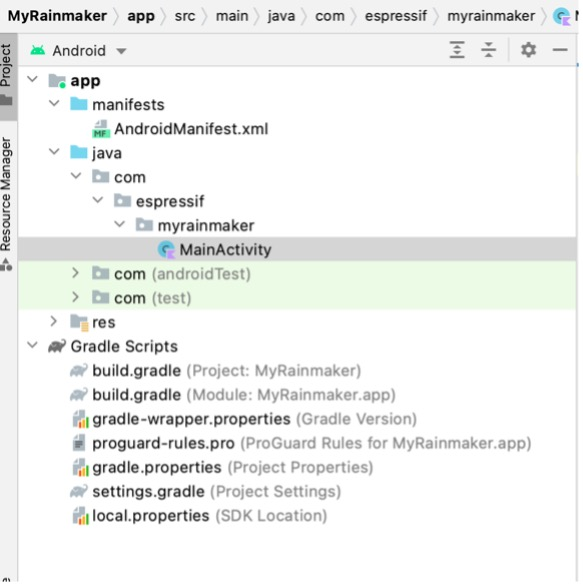
\includegraphics[width=0.4\textwidth,frame]{D10Z/10-1}
    \caption{Structure of the Android project}
\end{figure}

\begin{term}{\texttt{App} folder}
    The \verb|app| folder contains three subfolders: \verb|manifests|, \verb|java|, and \verb|res|.
    \begin{itemize}
        \item \verb|manifests|: Stores app configurations, including name, version, SDK, and permissions.
        \item \verb|java|: Mainly stores source code and test code.
        \item \verb|res|: Stores all project resources.
    \end{itemize}
\end{term}

\begin{term}{\texttt{Gradle Scripts} folder}
    The \verb|Gradle Scripts| folder contains \verb|build.gradle| (two files with the same name), \verb|gradle-wrapper.properties|, \verb|proguard-rules.pro|, \verb|gradle.properties|, \\ \verb|settings.gradle|, and \verb|local.properties|.
    \vspace{6pt}
    \begin{itemize}
        \item \verb|build.gradle|: Compiles the app with Gradle.
        \item \verb|gradle-wrapper.properties|: Configures the Gradle version.
        \item \verb|proguard-rules.pro|: Configures proguard rules to obfuscate the code.
        \item \verb|gradle.properties|: Configures Gradle-related global properties.
        \item \verb|settings.gradle|: Configures relevant Gradle scripts.
        \item \verb|local.properties|: Configures the path to the SDK/NDK.
    \end{itemize}
\end{term}

\subsection{Structure of the iOS Project}
This section takes MyRainmaker Apps an example to introduce the structure of an iOS project. As the navigation view shows in Figure 10.2, the project includes a \verb|MyRainmaker| folder for source code, a \verb|MyRainmakerTests| folder for unit test code, and a \verb|MyRainma-|\\
\verb|kerUITests| folder for UI test code.

\begin{figure}[ht]
    \centering
    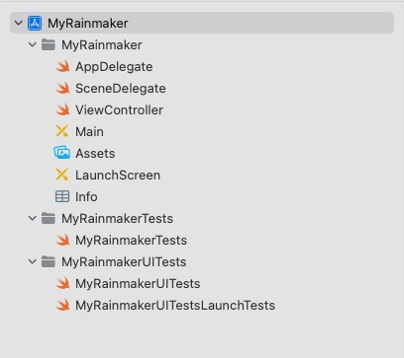
\includegraphics[width=0.55\textwidth]{D10Z/10-2}
    \caption{Structure of the iOS project}
\end{figure}

\begin{term}{\texttt{MyRainmaker} folder}
    This folder contains the \verb|AppDelegate|, \verb|SceneDelegate|, \verb|ViewController|, \verb|Main|, \verb|Assets|, \verb|LaunchScreen|, and \verb|Info| files.
    \vspace{6pt}
    \begin{itemize}
        \item \verb|AppDelegate|: The entry file of the entire app, which stores the app’s delegate class.
        \item \verb|SceneDelegate|: New class added to Xcode 11 that handles scenes split from AppDelegate.
        \item \verb|ViewController|: Host controller class that controls view display and handles touch events, etc.
        \item \verb|Main|: The main interface storyboard, which contains view controller scenes in the app and describes the connection between multiple view controllers.
        \item \verb|Assets|: The file that stores most images.
        \item \verb|LaunchScreen|: Configures the app’s launch screen.
        \item \verb|Info|: Configures app permissions, such as Bluetooth, location, and camera permissions.
    \end{itemize}
\end{term}

\begin{term}{Test files}
    \verb|MyRainmakerTests|, \verb|MyRainmakerUITests|, and \verb|MyRainmakerUITestsLaunch-|\\
    \verb|Tests| are all test classes. They are not commonly used in project development, and thus are not explained in detail.
\end{term}

\subsection{Lifecycle of an Android Activity}
Android has four basic components – Activity, Service, ContentProvider, and BroadcastReceiver, among which Activity is used very frequently and handles almost all interface interactions. Now, let’s explore the lifecycle of an activity following the Figure 10.3.

\begin{figure}[ht]
    \centering
    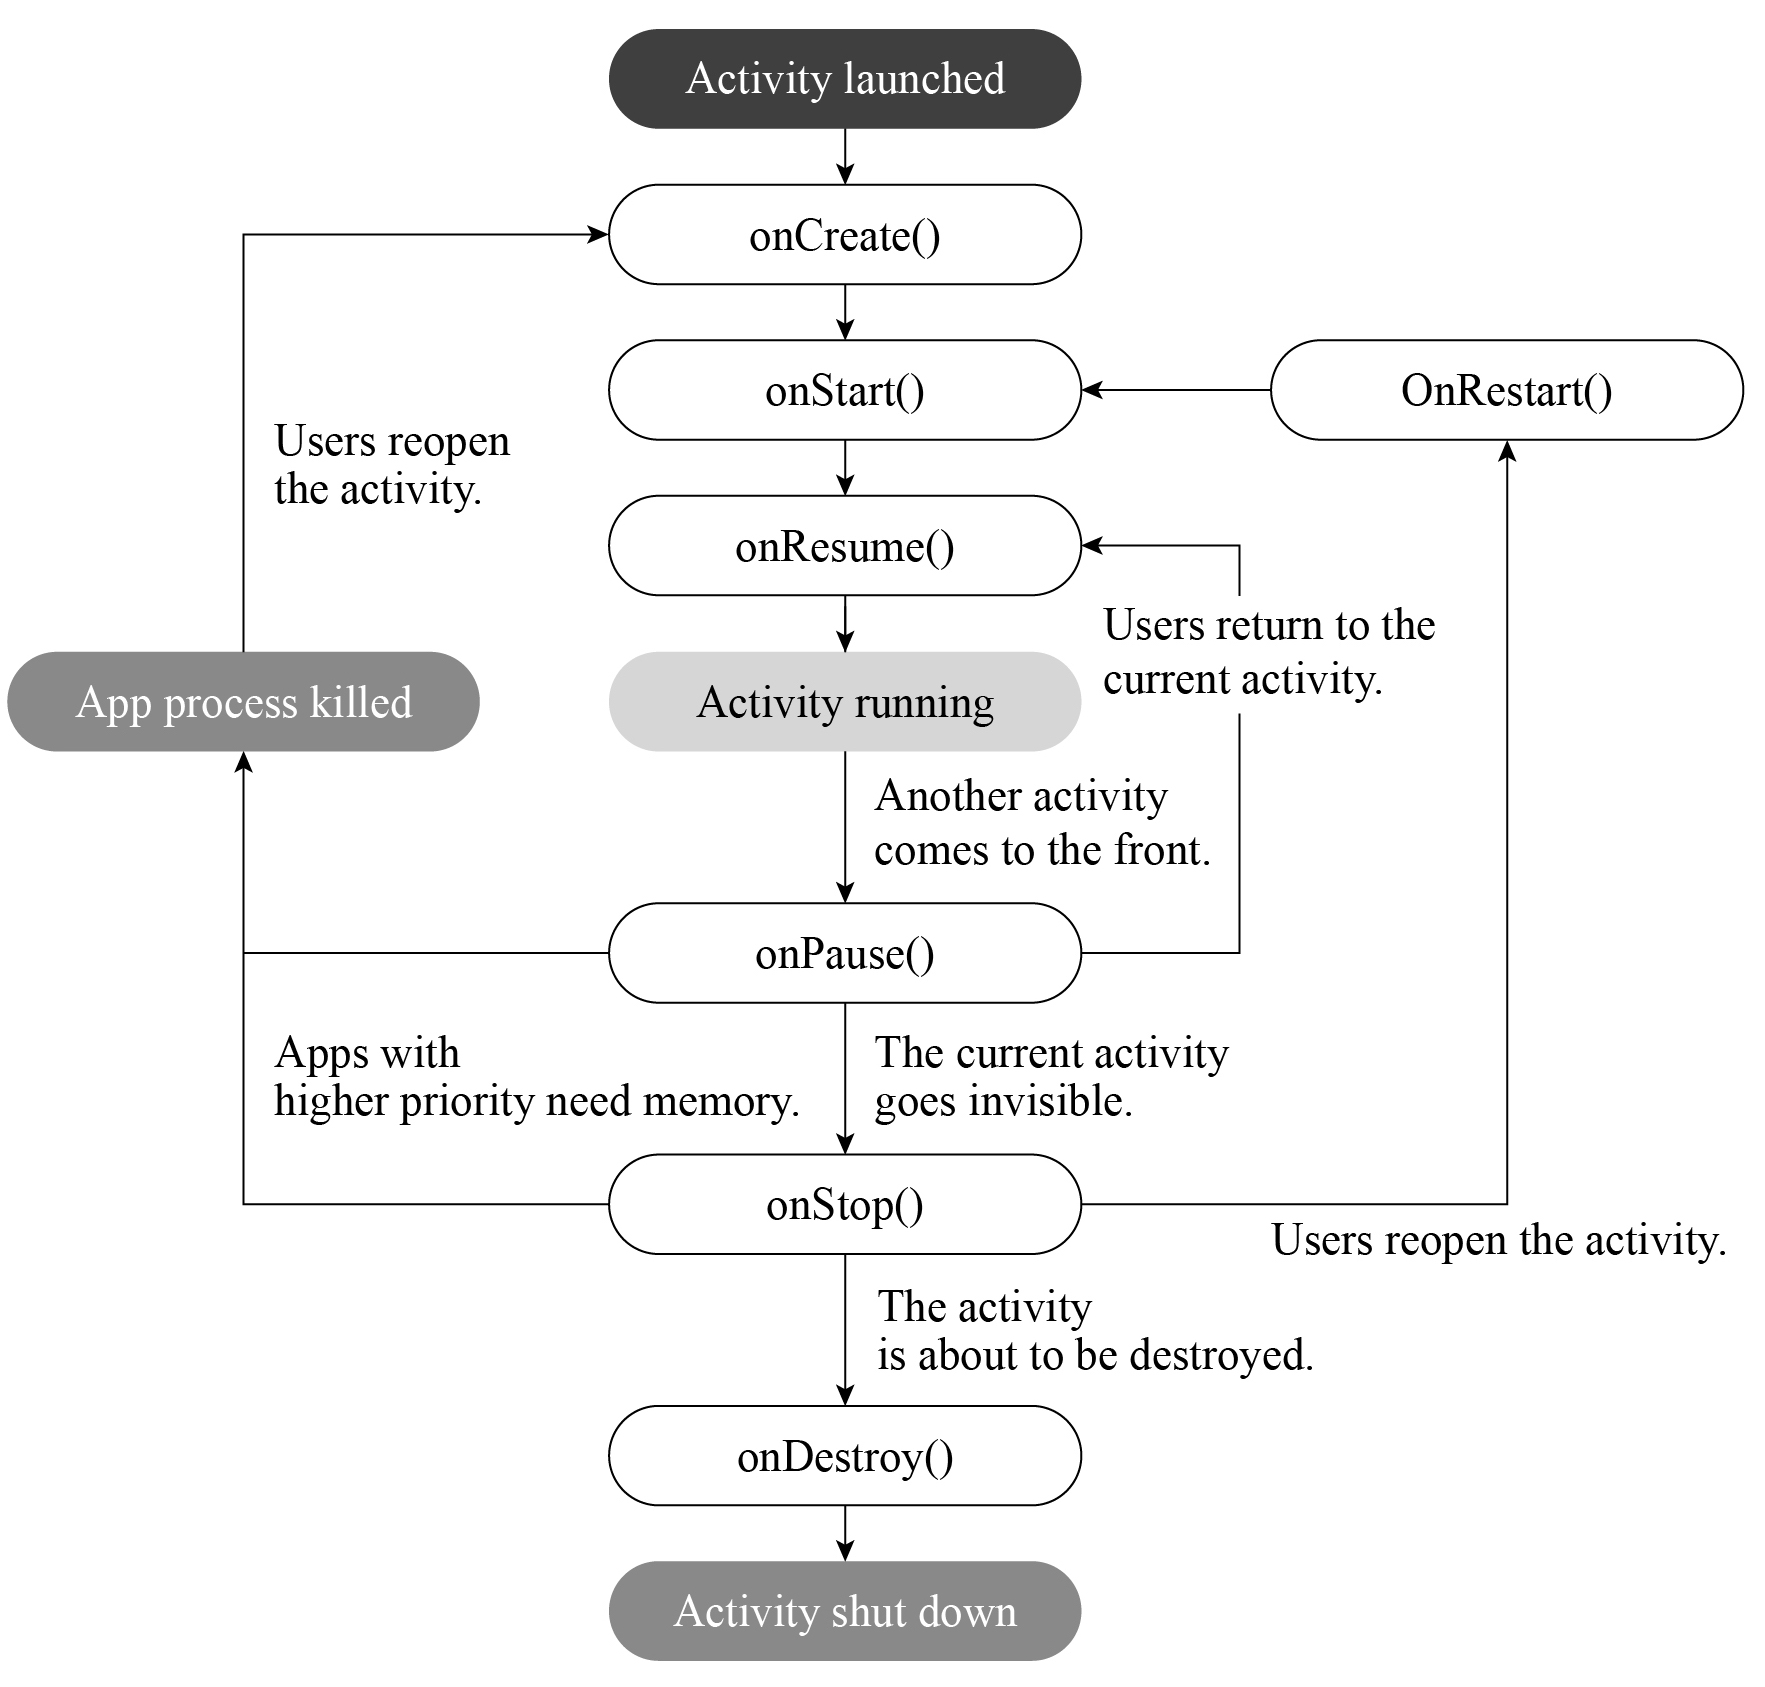
\includegraphics[width=0.73\textwidth]{D10Z/10-3}
    \caption{Lifecycle of an activity}
\end{figure}

\begin{itemize}
    \item \verb|onCreate()| indicates that the activity is being created. It is the first method through an activity’s lifecycle and is where you should do the initialization.
    \item \verb|onStart()| indicates that the activity is being started and is visible to users.
    \item \verb|onRestart()| indicates that the activity is being restarted, and should be called when the activity changes from invisible to visible. For example, when users press the Home button to switch to the desktop, or open a new activity, the current activity will be stopped. When the current activity returns to the front, the \verb|onRestart()| method will be called.
    \item \verb|onResume()| indicates that the activity has been created and users can operate and interact on the interface.
    \item \verb|onPause()| indicates that the activity is paused, and usually \verb|onStop()| will be called immediately after. If users quickly return to the current activity, \verb|onResume()| will be called.
    \item \verb|onStop()| indicates that the activity is about to stop. It is no longer visible to users and is running only in the background.
    \item \verb|onDestroy()| indicates that the activity is about to be destroyed. This is the last method executed in an activity’s lifecycle and is where you should reclaim or release resources.
\end{itemize}

\subsection{Lifecycle of iOS ViewController}
The lifecycle of the ViewController refers to the lifecycle of the views it controls. When the state of a view changes, the ViewController will automatically call a series of methods in response to the change. The lifecycle of the ViewController is shown in Figure 10.4.

\begin{figure}[ht]
    \centering
    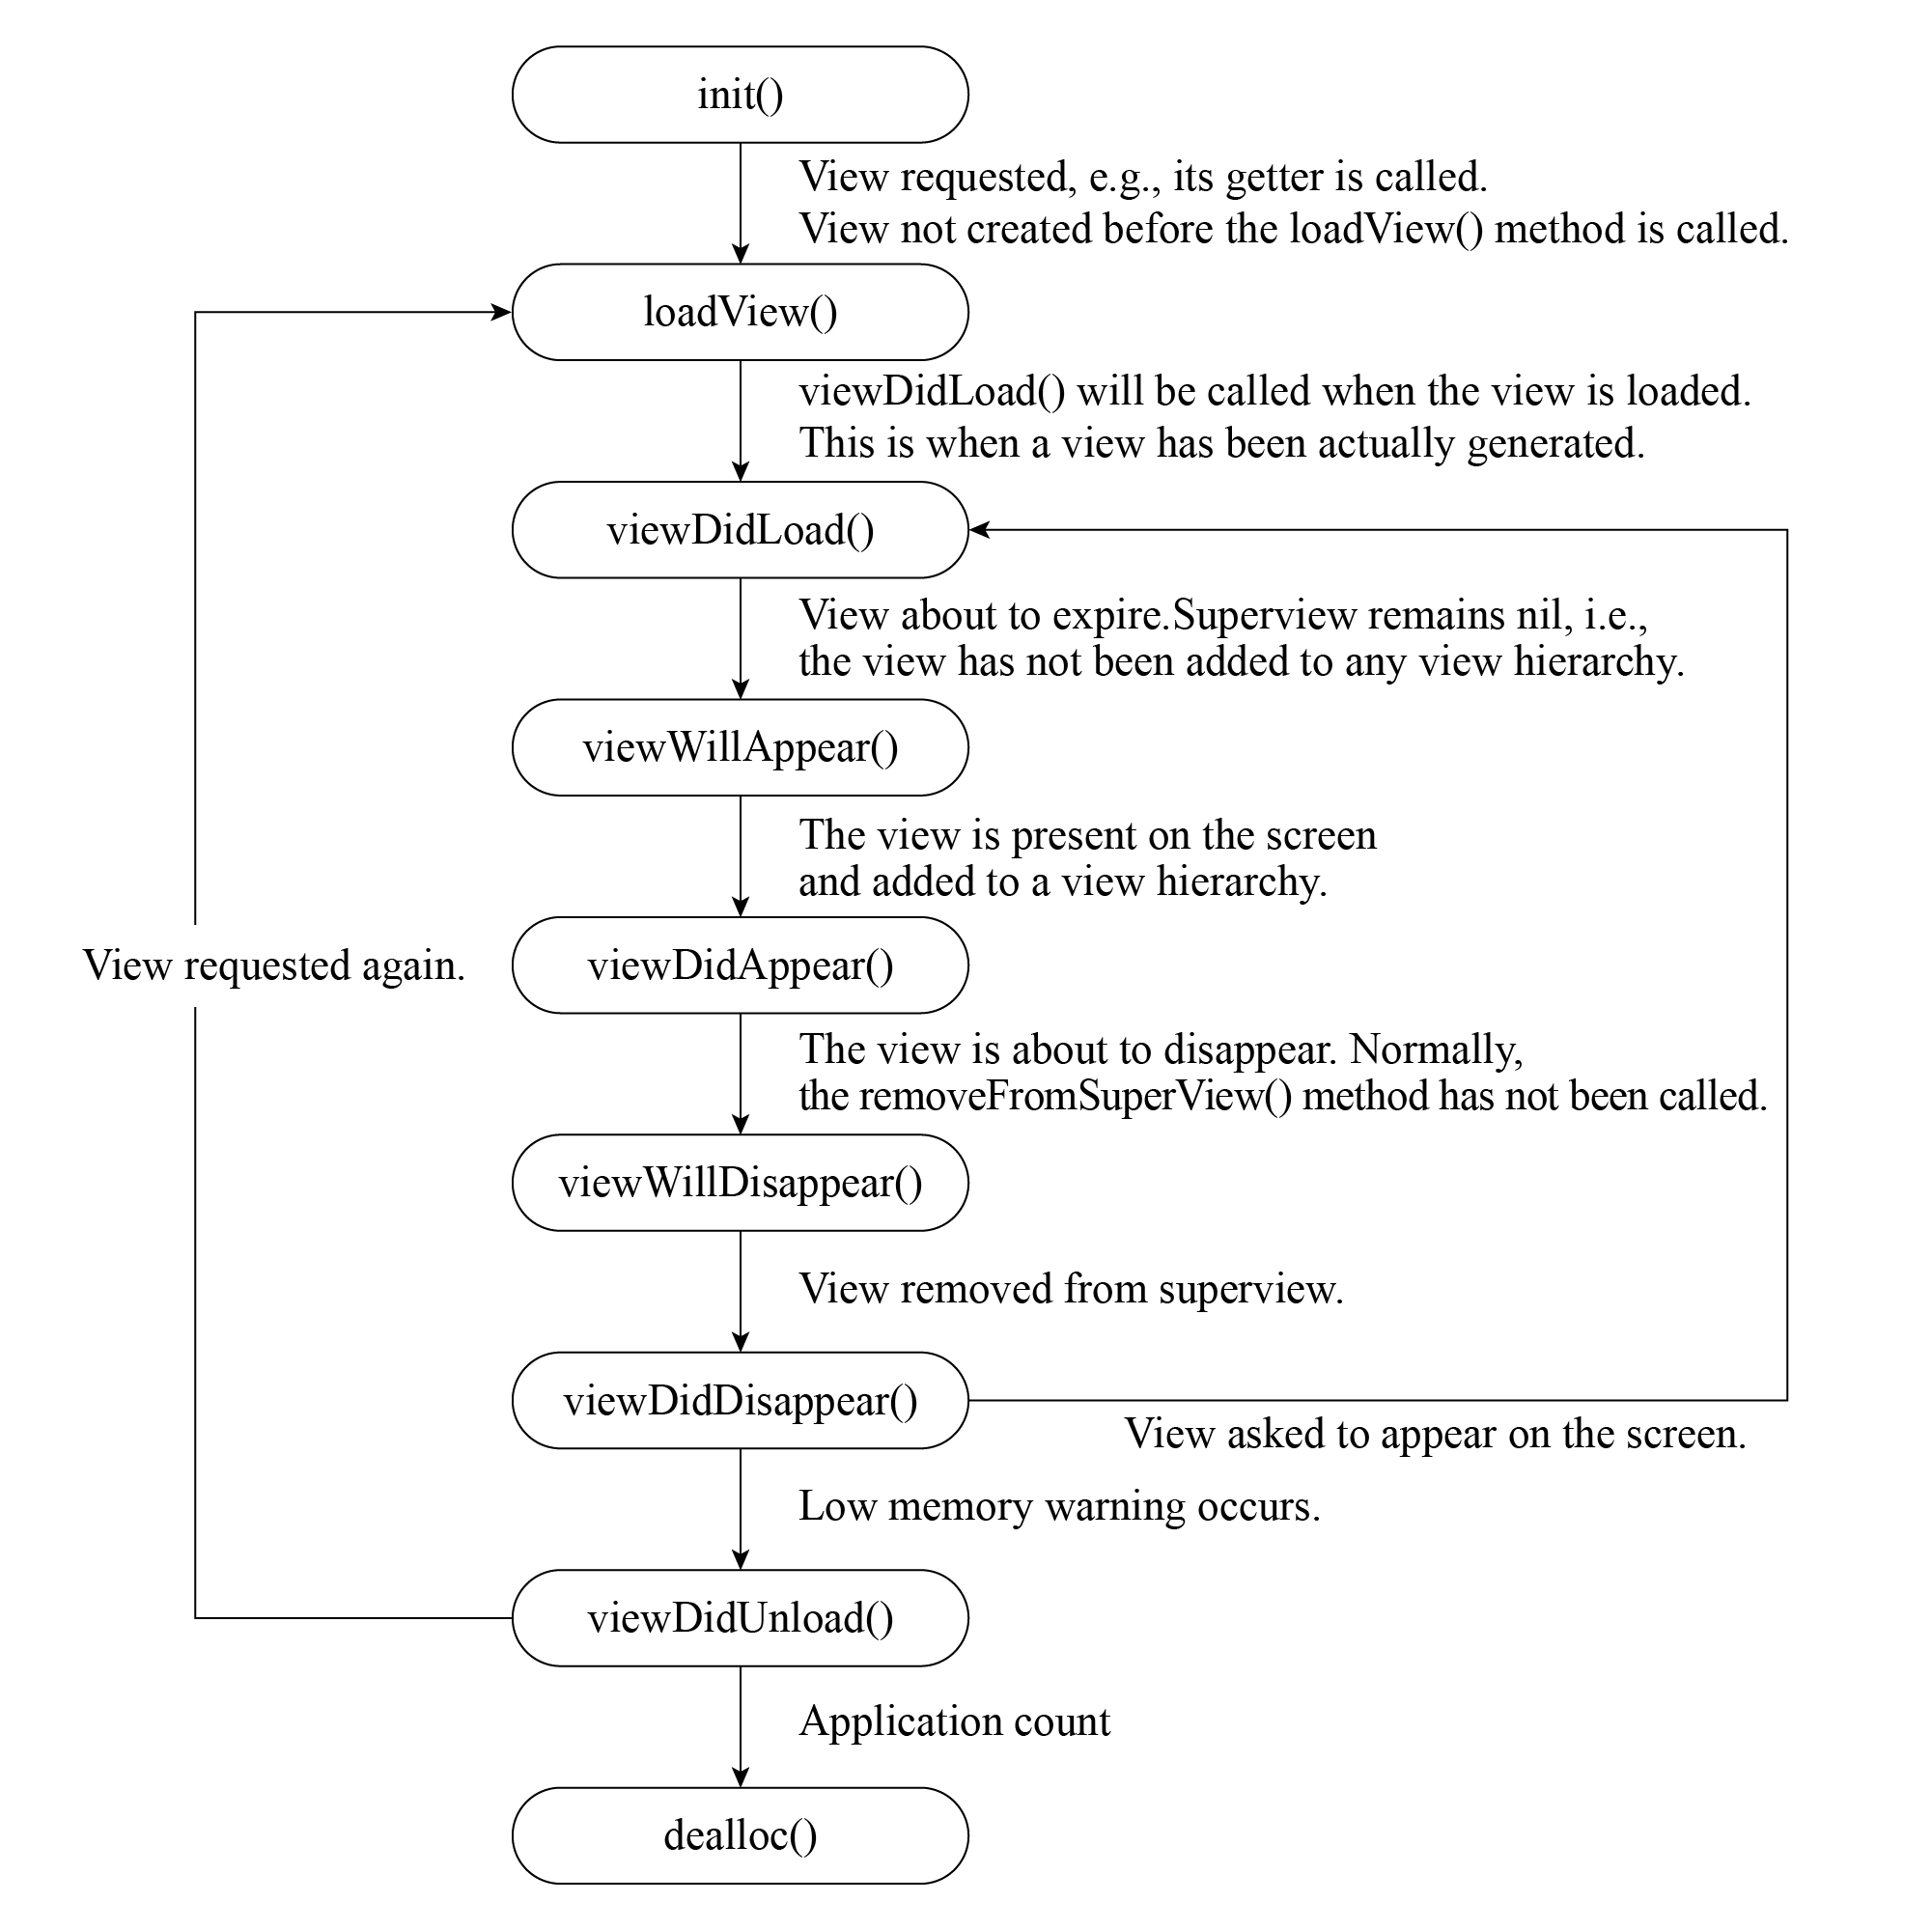
\includegraphics[width=0.85\textwidth]{D10Z/10-4}
    \caption{Lifecycle of ViewController}
\end{figure}

Each method is used as follows:

\begin{itemize}
    \item \verb|init()| initializes relevant, critical data.
    \item \verb|loadView()| initializes the view. This method should not be called directly, but automatically by the system.
    \item \verb|viewDidLoad()| indicates that the view is loaded, but not yet been displayed on the screen. By overriding this method, you can perform additional initialization on views, such as removing some views, modifying constraints, loading data, etc.
    \item \verb|viewWillAppear()| indicates that the view is about to be displayed on the screen. You may use this method to change the orientation or style of the status bar.
    \item \verb|viewDidApper()| indicates that the view has been displayed on the screen. You may use this method to modify how the view is presented.
    \item \verb|viewWillDisappear()| indicates that the view is about to disappear, be covered, or be hidden.
    \item \verb|viewDidDisappear()| indicates that the view has disappeared, been covered, or been hidden.
\end{itemize}

\section{Creating a New Smartphone App Project}
Now that we have learned about the development of Android and iOS project, let’s start creating a new app project. Since the provisioning function of the app requires a Bluetooth module, simulator does not meet the demand. Please prepare a smartphone for the development and debugging of the app.

Before creating a new smartphone app project, you need to download the corresponding development tools. IDE tools have integrated all the necessary environments, and do not require setting environment variables and other tedious work.

\subsection{Preparing for Android Development}
The Android app may be developed on Linux, Mac, or Windows using Android Studio. It should be targeted at Android 6.0 and above, and can be built with Java and Kotlin.

Kotlin is preferred for developing the Android app. As a JVM-oriented language, it is fully compatible with Java, and offers more flexible syntax and powerful features. Back in 2017, Google announced that it would support Kotlin on Android as a first-class language. With experience in Java development, you can easily get started with Kotlin.

\subsection{Creating a New Android Project}
To create a new Android project, proceed as follows:

After downloading and installing Android Studio on your PC, open it and you should see the interface as shown in Figure 10.5. Then click “New Project”.

\begin{figure}[ht]
    \centering
    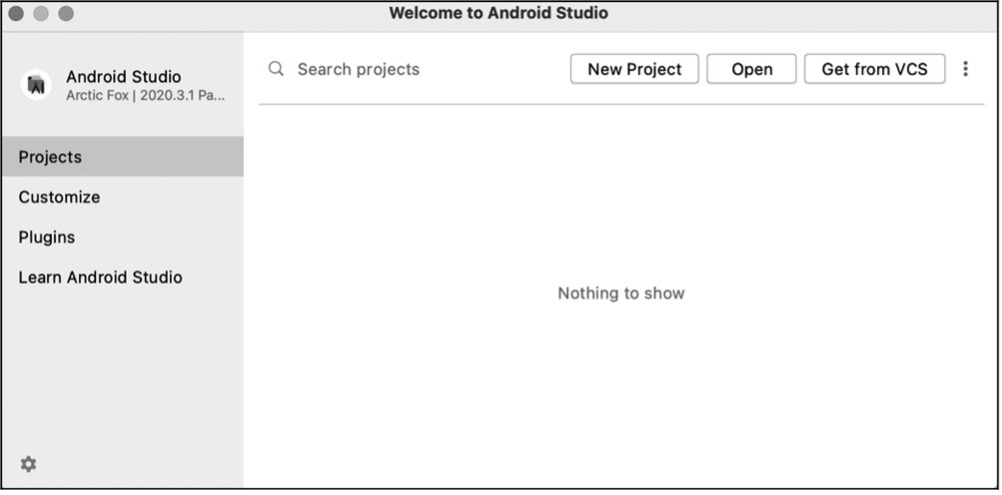
\includegraphics[width=0.9\textwidth]{D10Z/10-5}
    \caption{Interface of Android Studio}
\end{figure}

Select “Empty Activity”, click “Next”, and a “New Project” dialog box as Figure 10.6 will pop up. Specify the Name of your project (e.g., MyRainmaker) and the Package name, and set the Save location, the Language (Kotlin), and the Minimum SDK (Android 6.0 and above). Then click “Finish” to create a new project. 

When you create a project for the first time, it may take some time to automatically download all the dependencies, so please be patient.

\begin{figure}[ht]
    \centering
    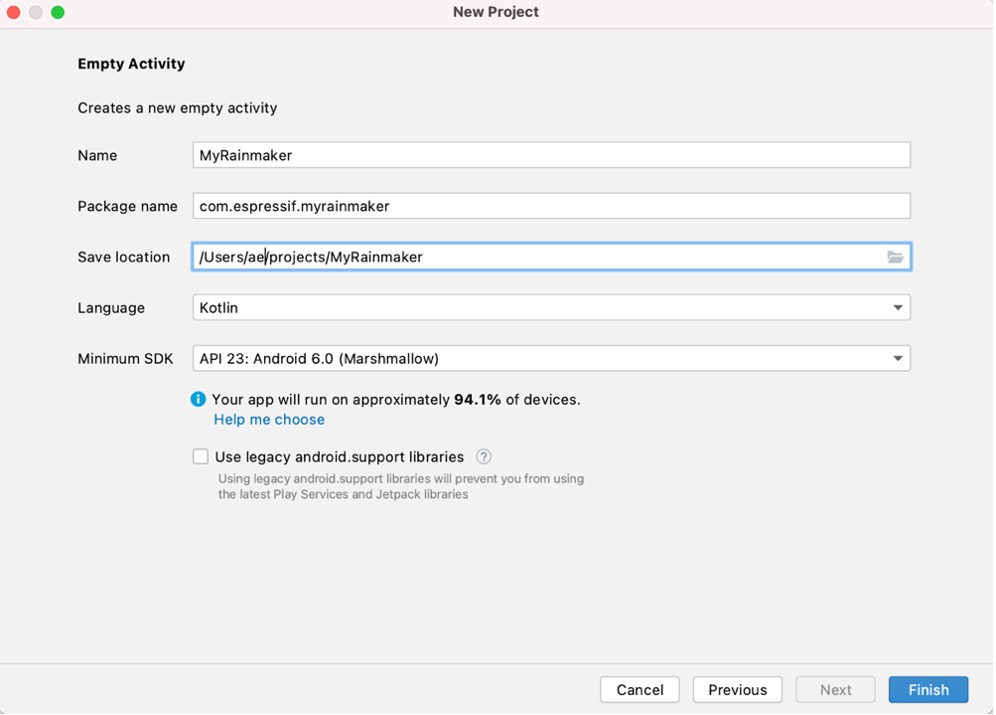
\includegraphics[width=0.8\textwidth,frame]{D10Z/10-6}
    \caption{The “New Project” dialog box}
\end{figure}

\subsection{Adding Dependencies for MyRainmaker}
Add repository to \verb|settings.gradle| (Project Settings).

\begin{codebloc}
\begin{tabular}{d}
\vspace{2pt}
\begin{verbatim}
1.  repositories {
2.      ...
3.      maven { url 'https://jitpack.io' }
\end{verbatim}
\verb|4.  }|
\end{tabular}
\end{codebloc}

Add dependencies to \verb|build.gradle| (Module: MyRainmaker.app).

\begin{codebloc}
\begin{tabular}{d}
\vspace{2pt}
\begin{verbatim}
1.  dependencies {
2.      implementation 'org.greenrobot:eventbus:3.2.0'
3.      implementation 'com.github.espressif:
4.                      esp-idf-provisioning-android:lib-2.0.11'
5.      implementation 'com.github.espressifApp:rainmaker-proto-java:1.0.0'
6.      implementation 'com.google.protobuf:protobuf-javalite:3.14.0'
7.      implementation 'com.google.crypto.tink:tink-android:1.6.1'
\end{verbatim}
\verb|8.  }|
\end{tabular}
\end{codebloc}

Click “Sync Now” or the “
\includegraphics[width=0.04\textwidth]{D10Z/sync}” (Sync) button in the upper right corner to download the dependencies, as shown in Figure 10.7.

\begin{figure}[ht]
    \centering
    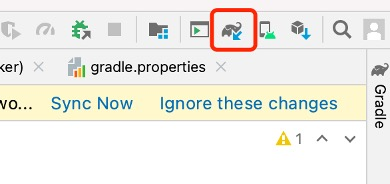
\includegraphics[width=0.53\textwidth,frame]{D10Z/10-7}
    \caption{Download dependencies}
\end{figure}

\subsection{Permission Request in Android}
Add the required permissions to the \verb|AndroidManifest.xml| file.

\begin{codebloc}
\begin{tabular}{d}
\vspace{2pt}
\begin{verbatim}
1. //Location permissions
2. <uses-permission android:name="android.permission.ACCESS_FINE_LOCATION" />
3. //Bluetooth permissions
4. <uses-permission android:name="android.permission.BLUETOOTH" />
5. <uses-permission android:name="android.permission.BLUETOOTH_ADMIN" />
6. //Network permissions
\end{verbatim}
\verb|7. <uses-permission android:name="android.permission.INTERNET" />|
\end{tabular}
\end{codebloc}

Besides being decalred as static, location permissions should also be requsted in the activity as follows:

\begin{codebloc}
\begin{tabular}{d}
\vspace{2pt}
\begin{verbatim}
1.  registerForActivityResult(ActivityResultContracts.RequestPermission()) 
2.  { granted ->
3.      //Result callback
4.      if (granted) {
5.          //Permission granted
6.      } else {
7.          //Permission denied
8.      }
\end{verbatim}
\verb|9.  }.launch(android.Manifest.permission.ACCESS_FINE_LOCATION)|
\end{tabular}
\end{codebloc}

Add the code above to the activity’s \verb|onCreate()| method, so that the app will request location permissions whenever being launched.

\subsection{Preparing for iOS Development}
The iOS app may be developed on computers runing macOS 10.12 and above using Xcode (available on App Store). It should be target at iOS 11.0 and above, and can be built with Swift and Objective-C.

Swift is preferred as it is faster, safer, and more interactive. It removes pointers and other unsafe access in Objective-C, and switches from the smalltalk-style syntax used by Objective-C to dot notation. All the sample code in this chapter is written in Swift.

\subsection{Creating a New iOS Project}
To create a new iOS project, proceed as follows:

After downloading and installing Xcode on your PC, open it, click “Create a new Xcode project”, select “iOS” → “App” as shown in Figure 10.8, and click “Next”. You should see a new prompt for your project details.

\begin{figure}[ht]
    \centering
    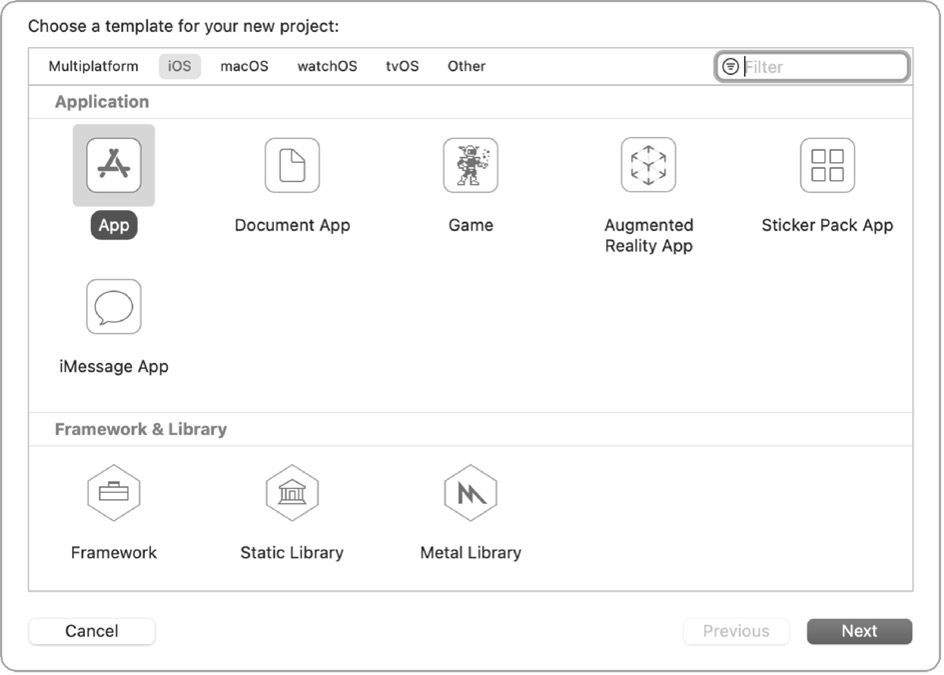
\includegraphics[width=0.63\textwidth]{D10Z/10-8}
    \caption{Select “iOS” → “App”}
\end{figure}

\begin{figure}[h!]
    \centering
    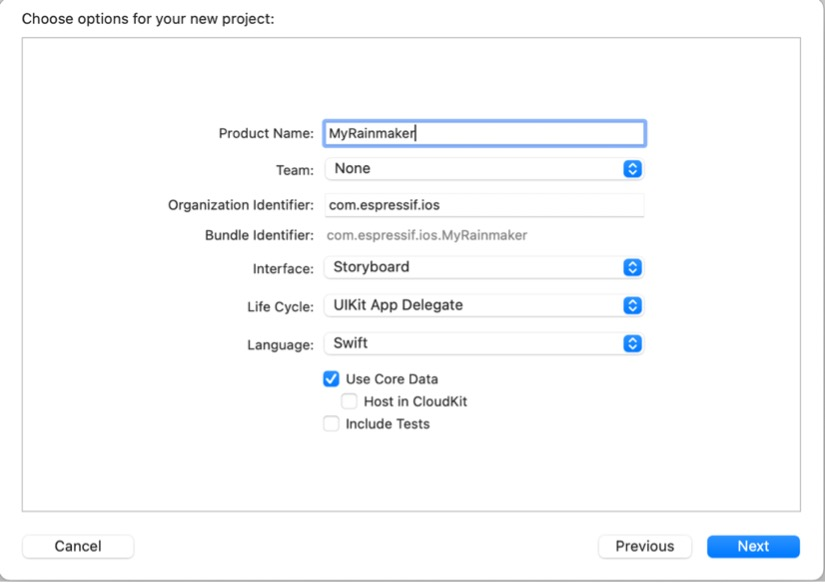
\includegraphics[width=0.63\textwidth,frame]{D10Z/10-9}
    \caption{Set project details}
\end{figure}

Set the Product Name (e.g., MyRainmaker), Team, Organization Identifier, Interface, Life Cycle, and Language (Swift), as shown in Figure 10.9. Click “Next”, and you should see a prompt for the project’s location. Set the storage path and click “Create”.

\subsection{Adding Dependencies for MyRainmaker}
Open the terminal, navigate to the project directory, and execute the following command to generate a \verb|Podfile|.

\begin{codebloc}
\begin{tabular}{d}
\% \textbf{touch Podfile}
\end{tabular}
\end{codebloc}

Open the \verb|Podfile| and add dependencies.

\begin{codebloc}
\begin{tabular}{d}
\vspace{2pt}
\begin{verbatim}
1.  # Uncomment the next line to define a global platform for your project
2.  platform :ios, '12.0'
3.
4.  target 'ESPRainMaker' do
5.      # Comment the next line if you're not using Swift and don't want to
6.      use dynamic frameworks
7.      use_frameworks!
8.
9.      # Pods for ESPRainMaker
10.
11.     pod 'MBProgressHUD', '~> 1.1.0'
12.     pod 'Alamofire', '~> 5.0.0'
13.     pod 'Toast-Swift'
14.     pod 'ReachabilitySwift'
15.     pod 'JWTDecode', '~> 2.4'
16.     pod 'M13Checkbox'
17.     pod 'ESPProvision'
18.     pod 'DropDown'
19.     pod 'FlexColorPicker'
20.
21. end
22.
23. post_install do |installer|
24.     .pods_project.targets.each do |target|
25.         target.build_configurations.each do |config|
26.             config.build_settings['IPHONEOS_DEPLOYMENT_TARGET'] = '12.0'
27.         end
28.     end
\end{verbatim}
\verb|29. end|
\end{tabular}
\end{codebloc}

Execute the following command to download dependencies.

\begin{codebloc}
\begin{tabular}{d}
\% \textbf{pod install}
\end{tabular}
\end{codebloc}

After download, open the project folder and double-click \verb|MyRainmaker.xcworkspace| to open the project, as shown in Figure 10.10.

\begin{figure}[ht]
    \centering
    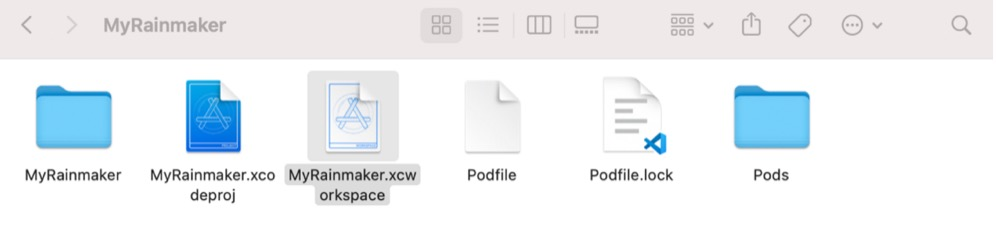
\includegraphics[width=0.7\textwidth,frame]{D10Z/10-10}
    \caption{Double-click \texttt{MyRainmaker.xcworkspace}}
\end{figure}

The structure of the project is shown in Figure 10.11.

\begin{figure}[h!]
    \centering
    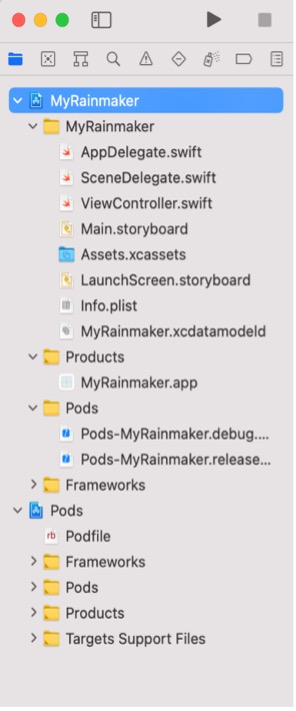
\includegraphics[width=0.25\textwidth]{D10Z/10-11}
    \caption{Structure of the project}
\end{figure}

\subsection{Permission Request in iOS}
Add the following permissions to \verb|info.plist| in the \verb|MyRainmaker| folder.

\begin{itemize}
    \item \verb|key NSBluetoothAlways Usage Description| and \verb|key NSBluetooth|\\
    \verb|Peripheral UsageDescription| for Bluetooth permission.
    \item \verb|key NSCamera Usage Description| for camera permission to scan QR codes.
    \item \verb|key NSLocationWhenInUseUsage Description| for location permission. (It is required for devices running iOS 13 and above to access SSID.)
    \item \verb|key NSLocalNetworkUsageDescription| for local network permission. (It is required for devices running iOS 14 and above to communicate over local network.)
\end{itemize}

\section{Analysis of the App’s Functional Requirements}
In the previous sections, we have introduced how to create a new app project, along with its structure and lifecycle. Now, to help you understand the development of app functionalities more concretely, we have included the source code of the smartphone app project in our GitHub, and you can import it into Android Studio/Xcode to run for for reference.

The main function of the smartphone app is to configure devices developed based on Espressif’s chips and modules to a designated router, and send commands through the app to control these devices, such as smart lights and sensors. Another function is to set the device status at a specified time using the scheduling module, for example, to turn on the water heater on the way home, so that hot water will be available as soon as you arrive.

\begin{figure}[ht]
    \centering
    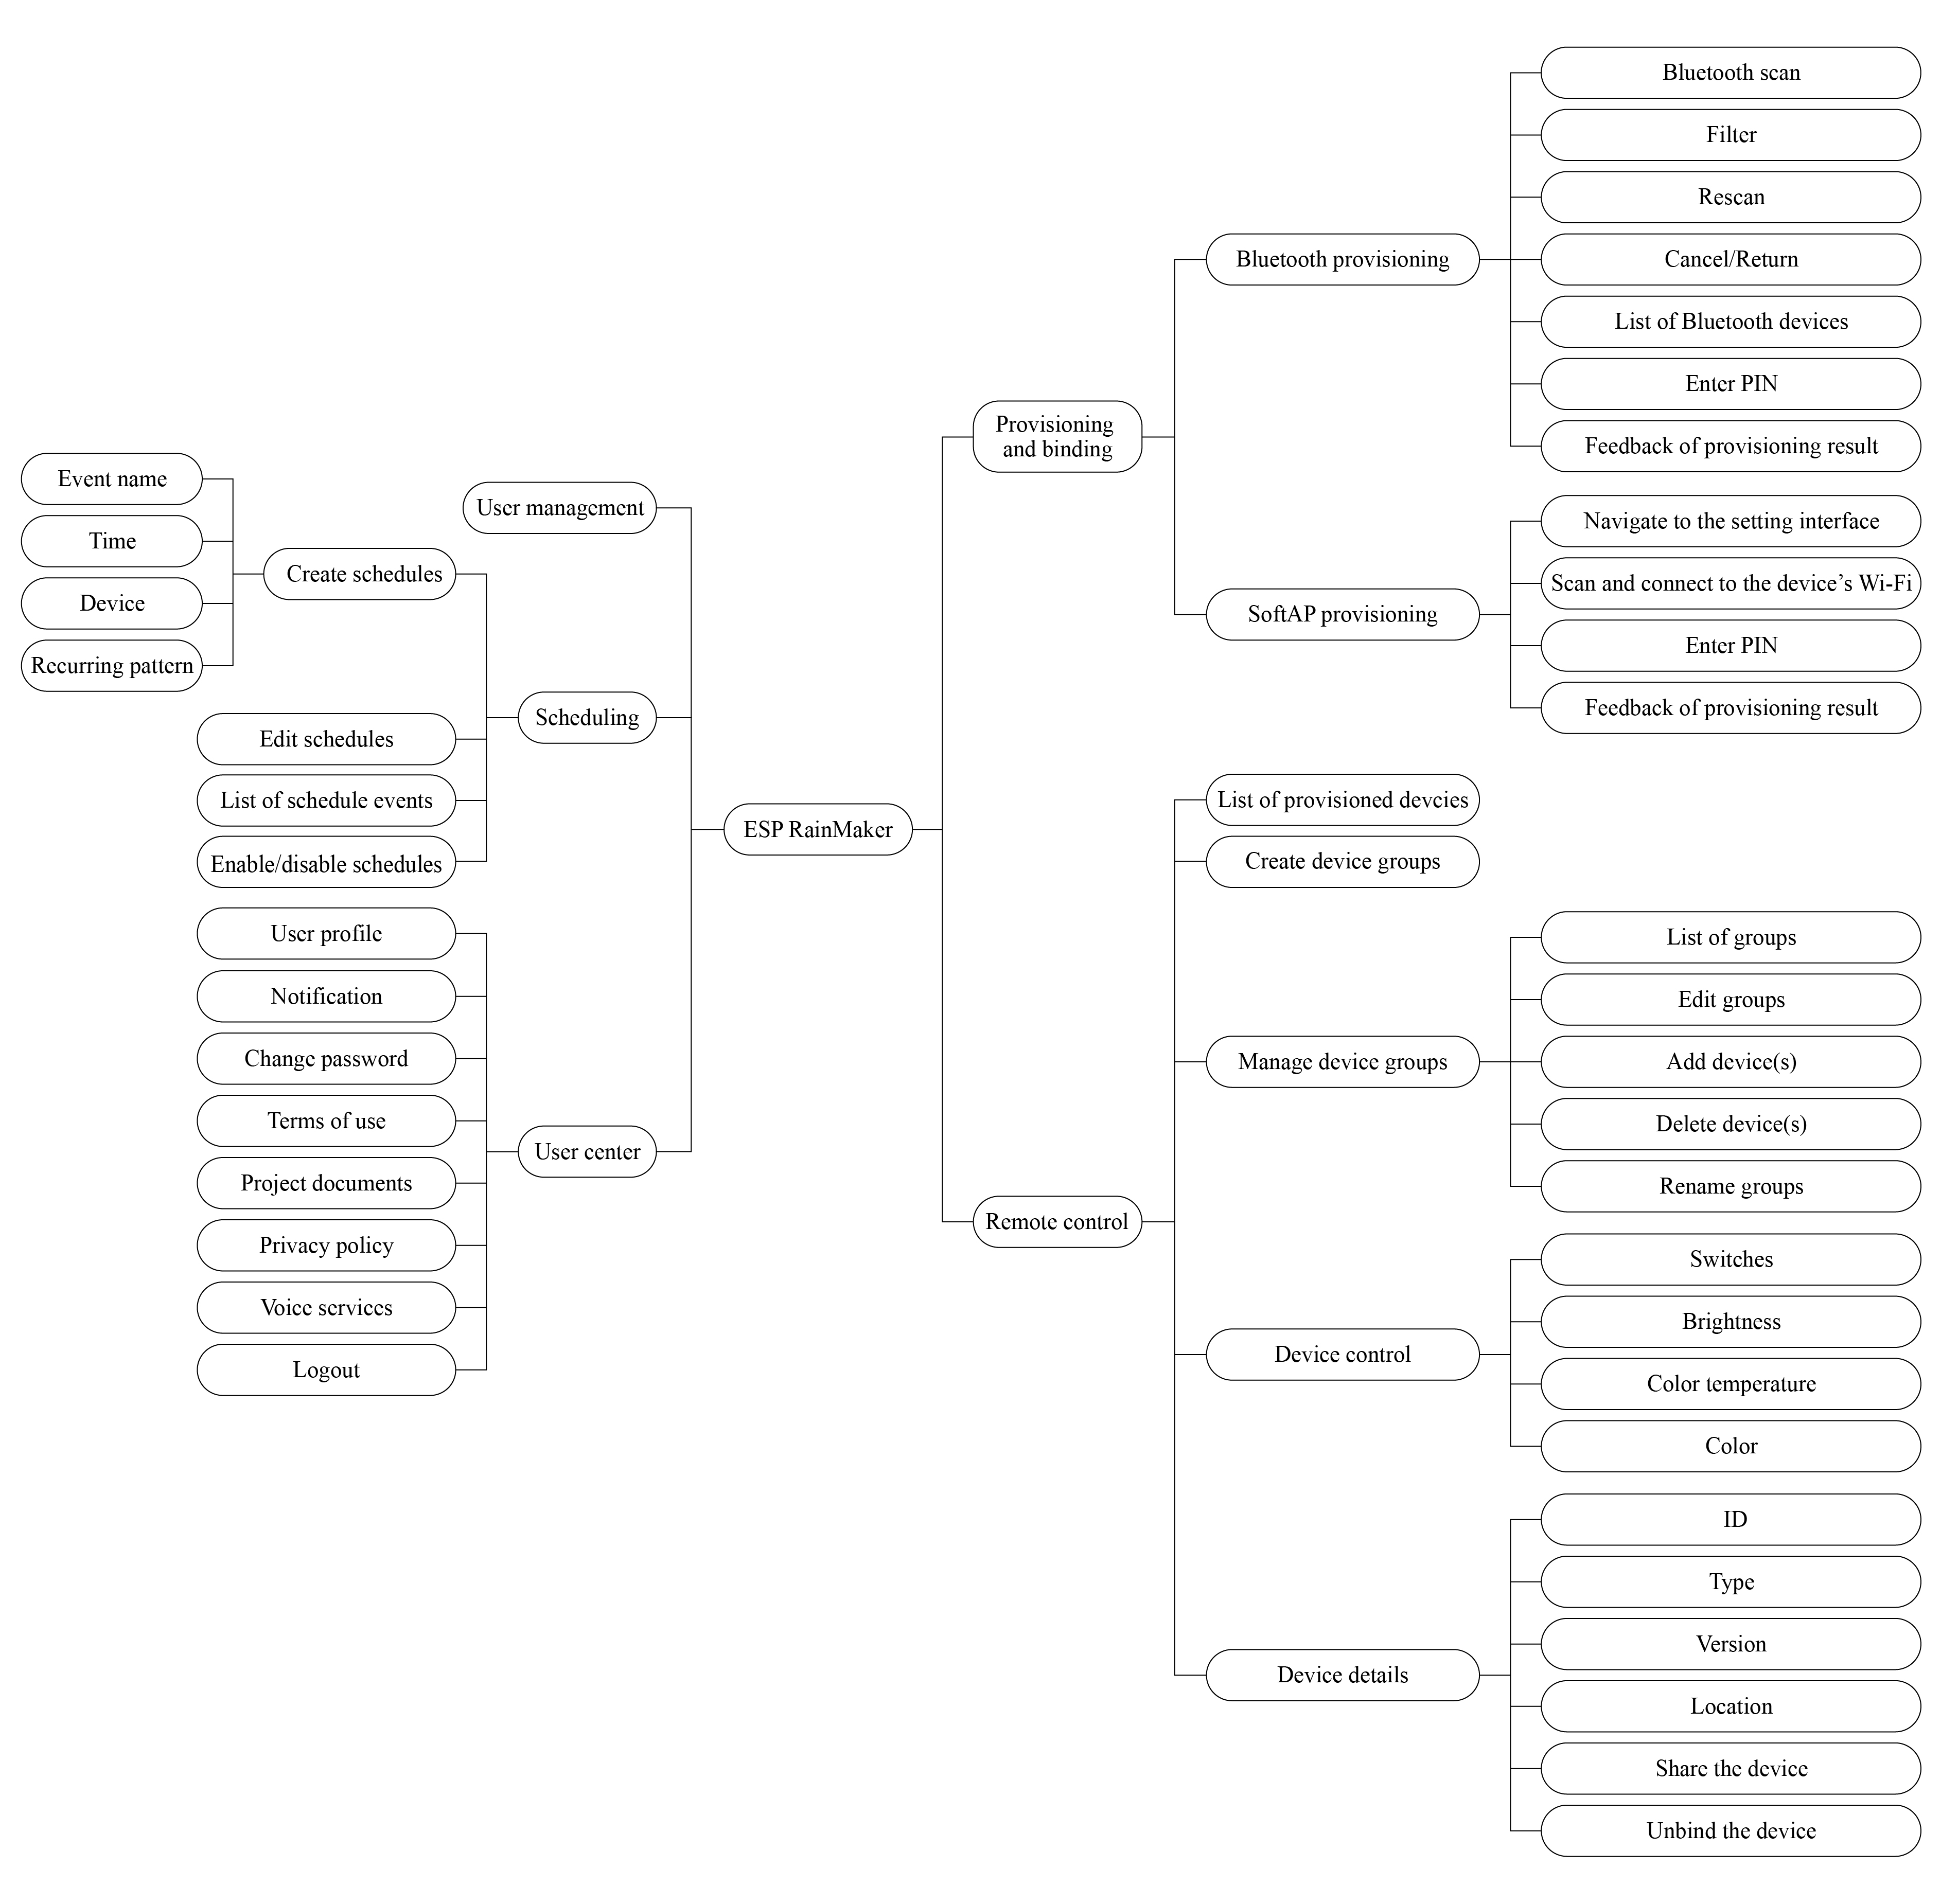
\includegraphics[width=0.9\textwidth]{D10Z/10-12}
    \caption{Functional requirements of the project}
\end{figure}

\subsection{Analysis of the Project’s Functional Requirements}
Before developing the app, you should first understand the functional modules and specific functions to be implemented in this project. The smartphone app project in this chapter mainly includes modules such as user management, provisioning, and device control (more functions illustrated in Figure 10.12). The following sections will provide a module-by-module breakdown.

\subsection{Analysis of User Management Requirements}
User registration and login are implemented in one interface and switched through the toggle button. The critical part of this module is to allow third-party accounts, and the network requests for registration, login, verification code acquisition, etc., and data parsing. The analysis of user management requirements is shown in Figure 10.13.

\begin{figure}[ht]
    \centering
    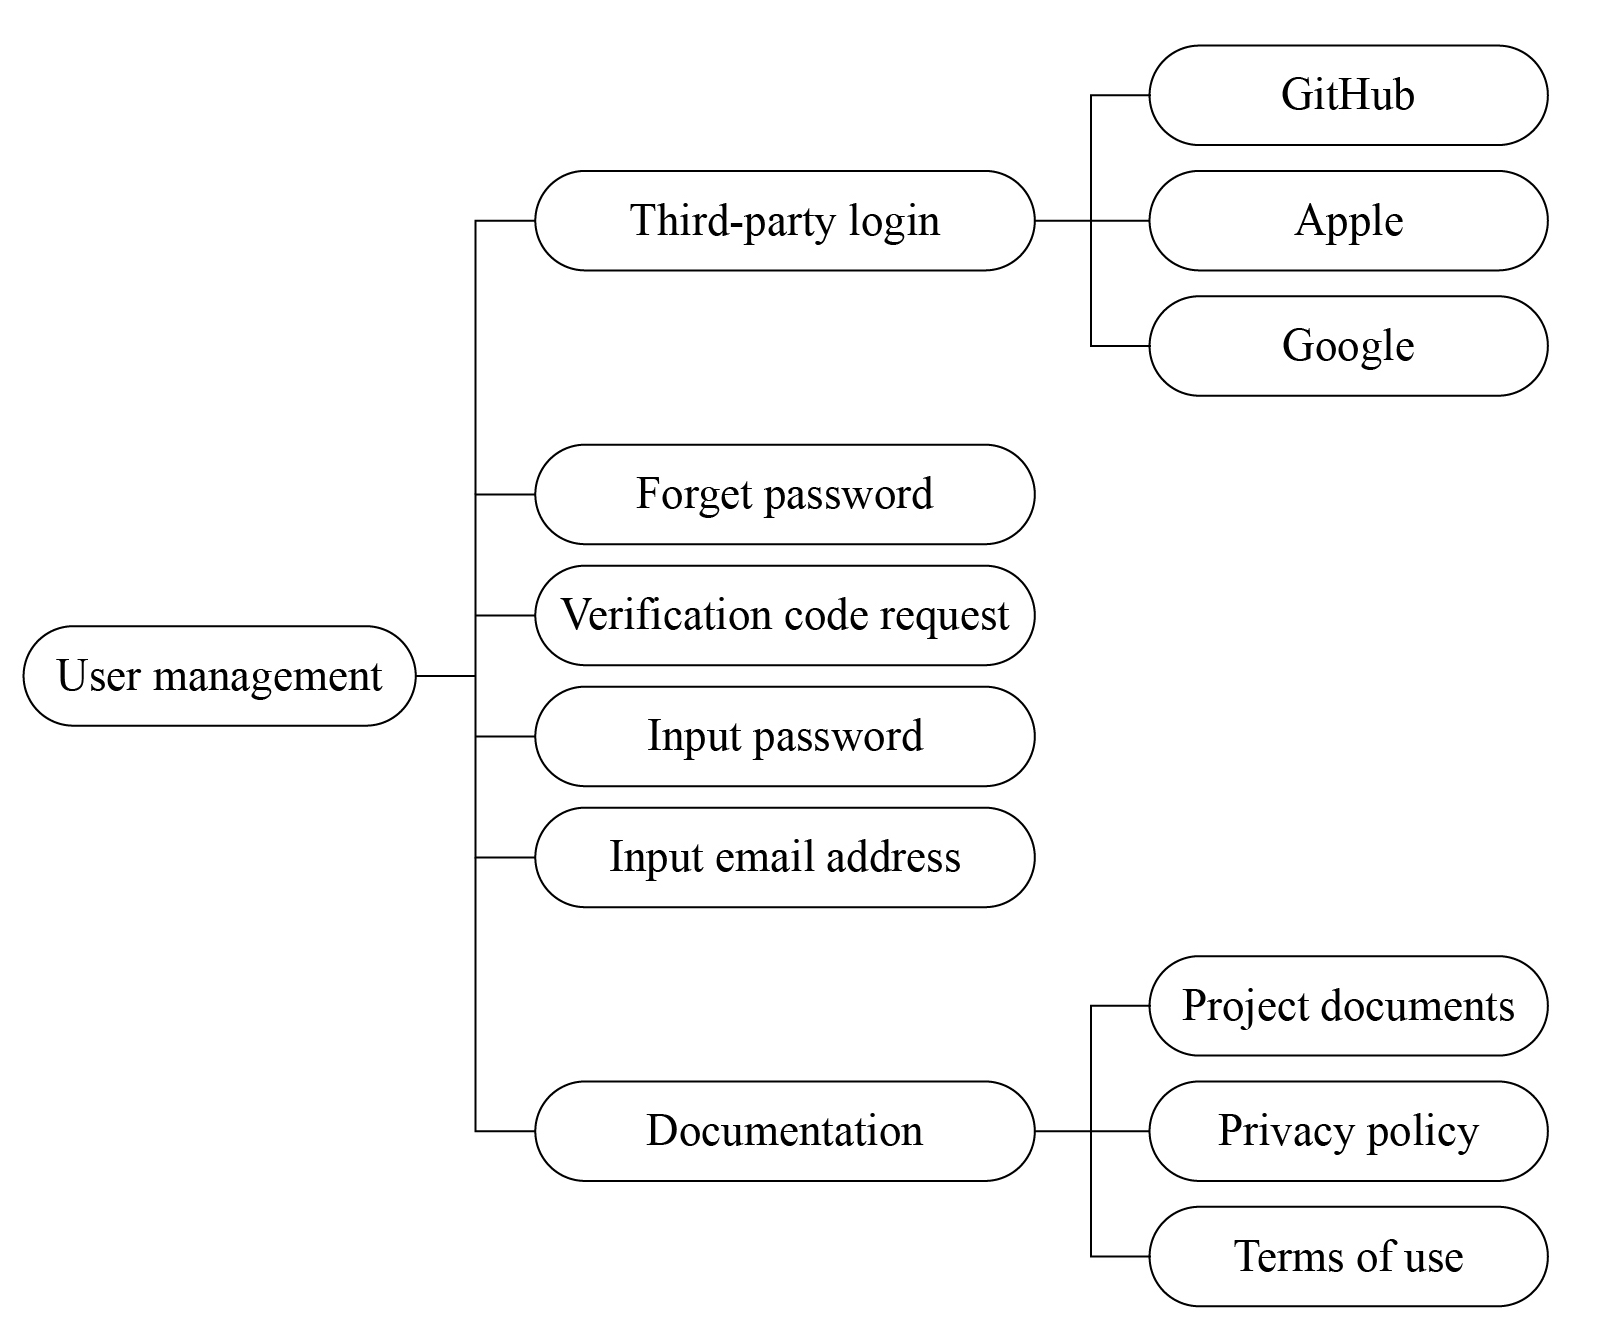
\includegraphics[width=0.55\textwidth]{D10Z/10-13}
    \caption{Analysis of user management requirements}
\end{figure}

\begin{itemize}
    \item To log in with a third-party account such as GitHub, Apple, or Google, the app will first open a webpage in the browser and obtain the unique identifier of the account.
    \item Forgot password and verification code request can be implemented via corresponding cloud APIs.
    \item Passwords entered will be displayed by default in ciphertext and can be switched to plaintext for confirmation by clicking the toggle (eye icon).
    \item Email addresses entered will be validated using regular expressions.
    \item Documentation will include documents for the entire project and can be accessed from various places in the app.
\end{itemize}

\subsection{Analysis of Device Provisioning and Binding Requirements}
There are two ways to provision a device. One is \textbf{Bluetooth provisioning}, where the app connects and communicates with the device through Bluetooth, provides provisioning data for the device, and allows it to join the network. Another way is \textbf{SoftAP provisioning}, where the device starts a \textbf{Wi-Fi hotspot} for the smartphone to connect and communicate with each other. Once the device is provisioned, enter PIN to bind the device over cloud. The analysis of device provisioning and binding requirements is shown in Figure 10.14.

\begin{figure}[ht]
    \centering
    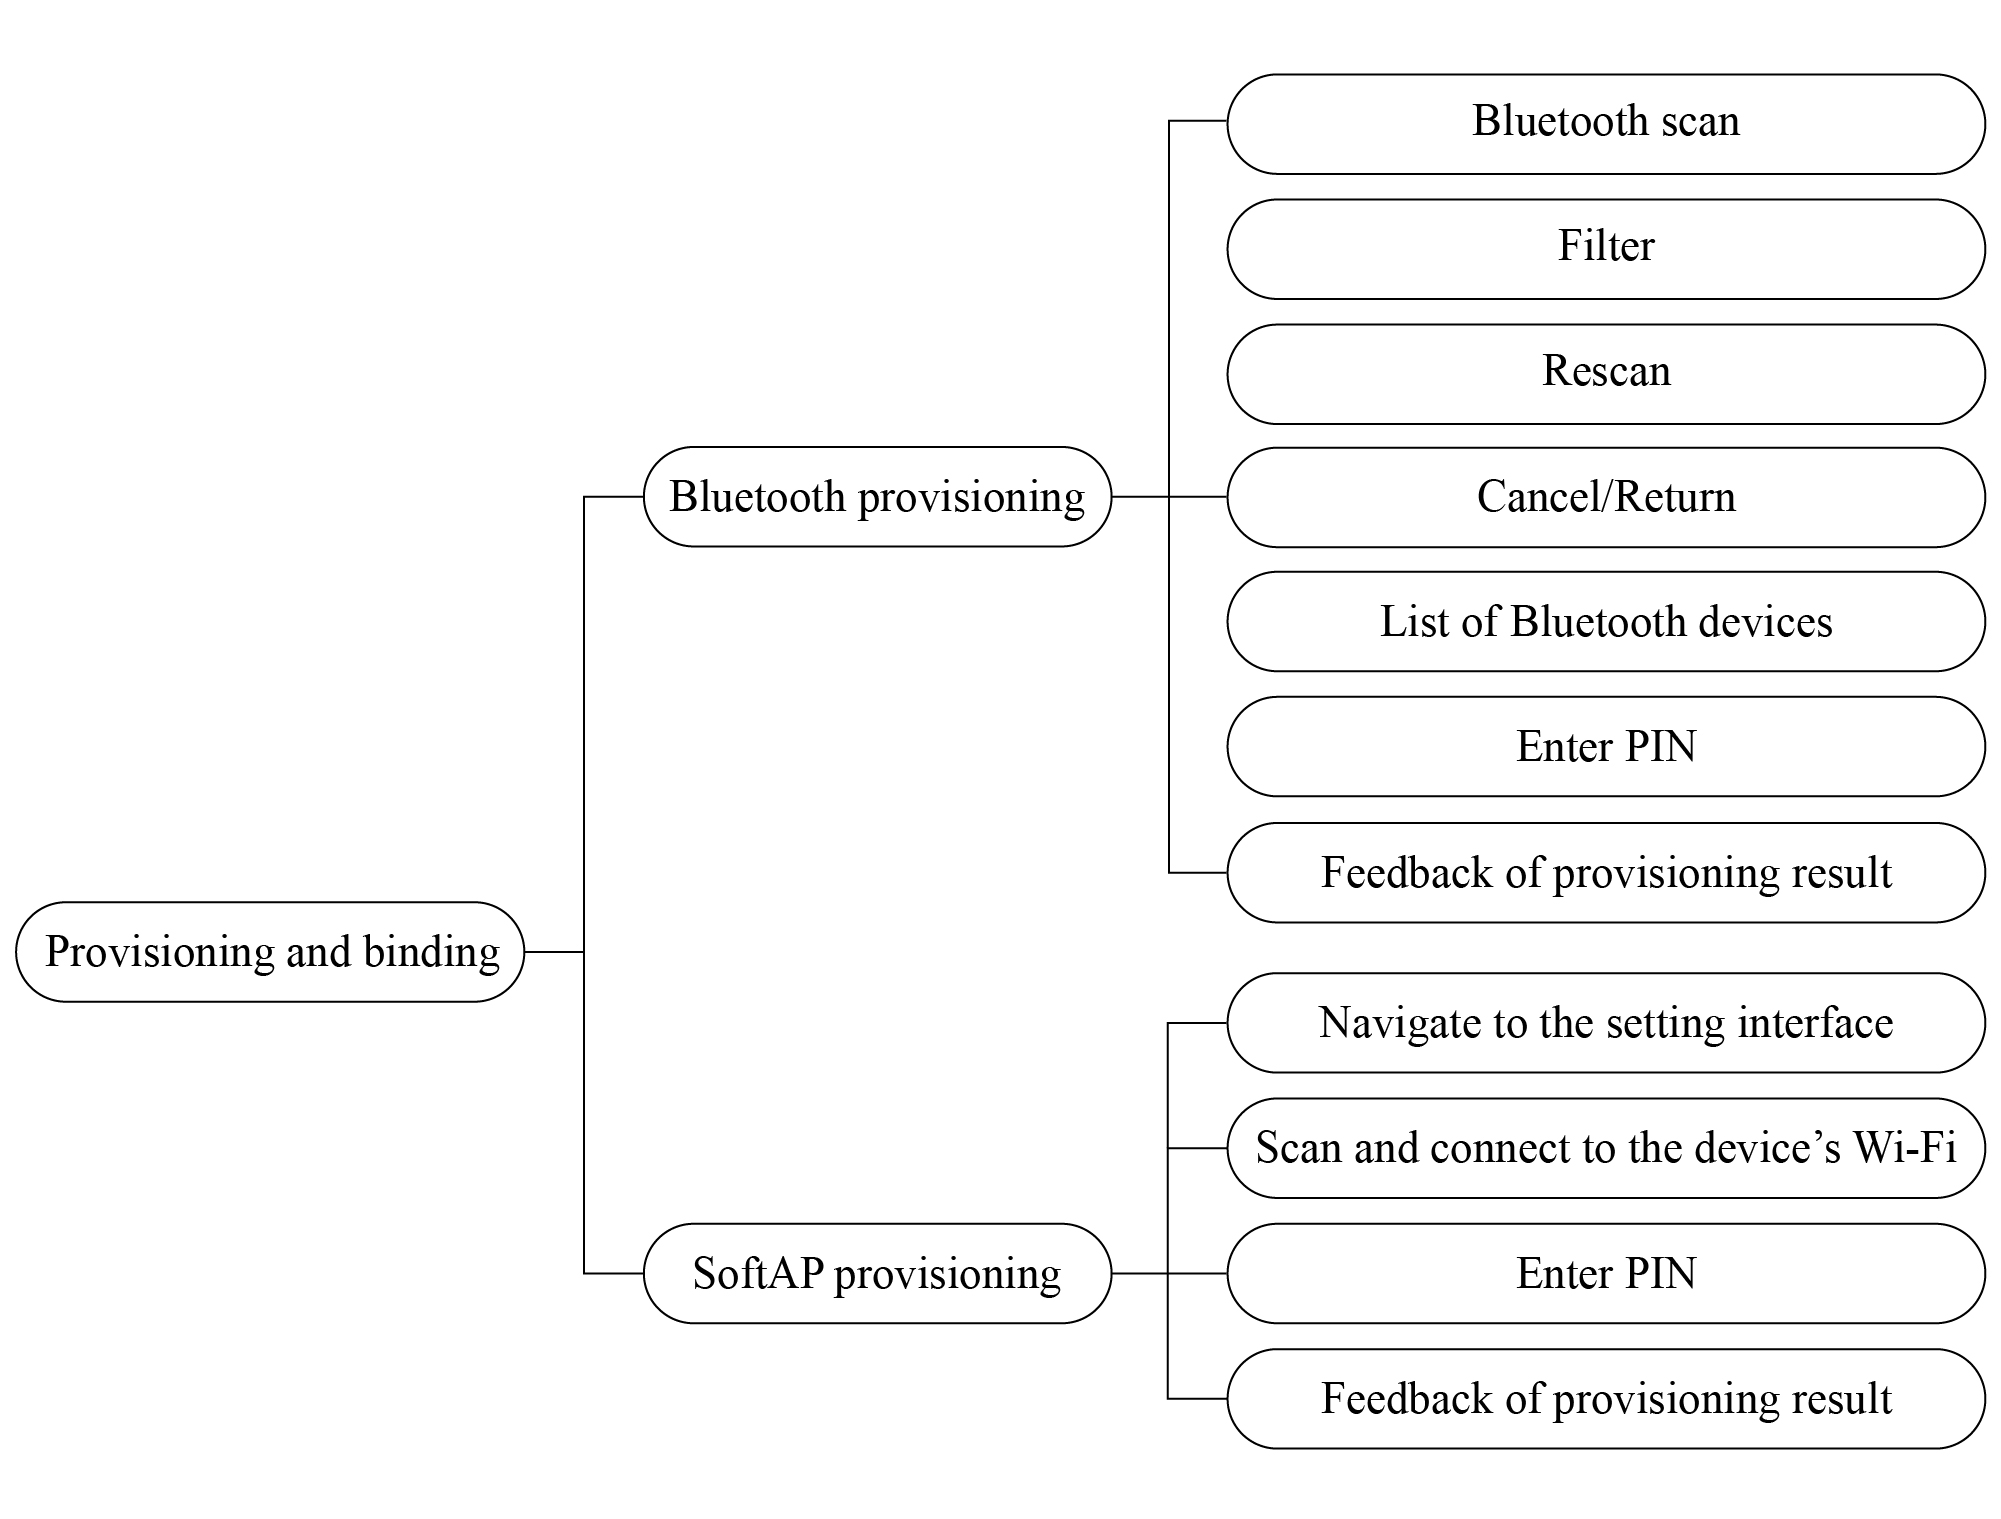
\includegraphics[width=0.6\textwidth]{D10Z/10-14}
    \caption{Analysis of device provisioning and binding requirements}
\end{figure}

\begin{itemize}
    \item For Bluetooth provisioning, the app needs to implement Bluetooth scanning, connection, subscription, packet transmission and other functions.
    \item For SoftAP provisioning, the app needs to navigate to the system setting interface, connect to the device’s Wi-Fi hotspot, and display information about the connected Wi-Fi hotspot.
    \item The implementation of device binding after provisioning is the same for both ways and can be reused.
\end{itemize}

\subsection{Analysis of Remote-Control Requirements}
Once the device gets provisioned and bound, users will be able to use the smartphone app to monitor and control it remotely. In addition, users can also control multiple devices at the same time and create groups to manage them. The analysis of remote-control requirements is shown in Figure 10.15.

\begin{figure}[ht]
    \centering
    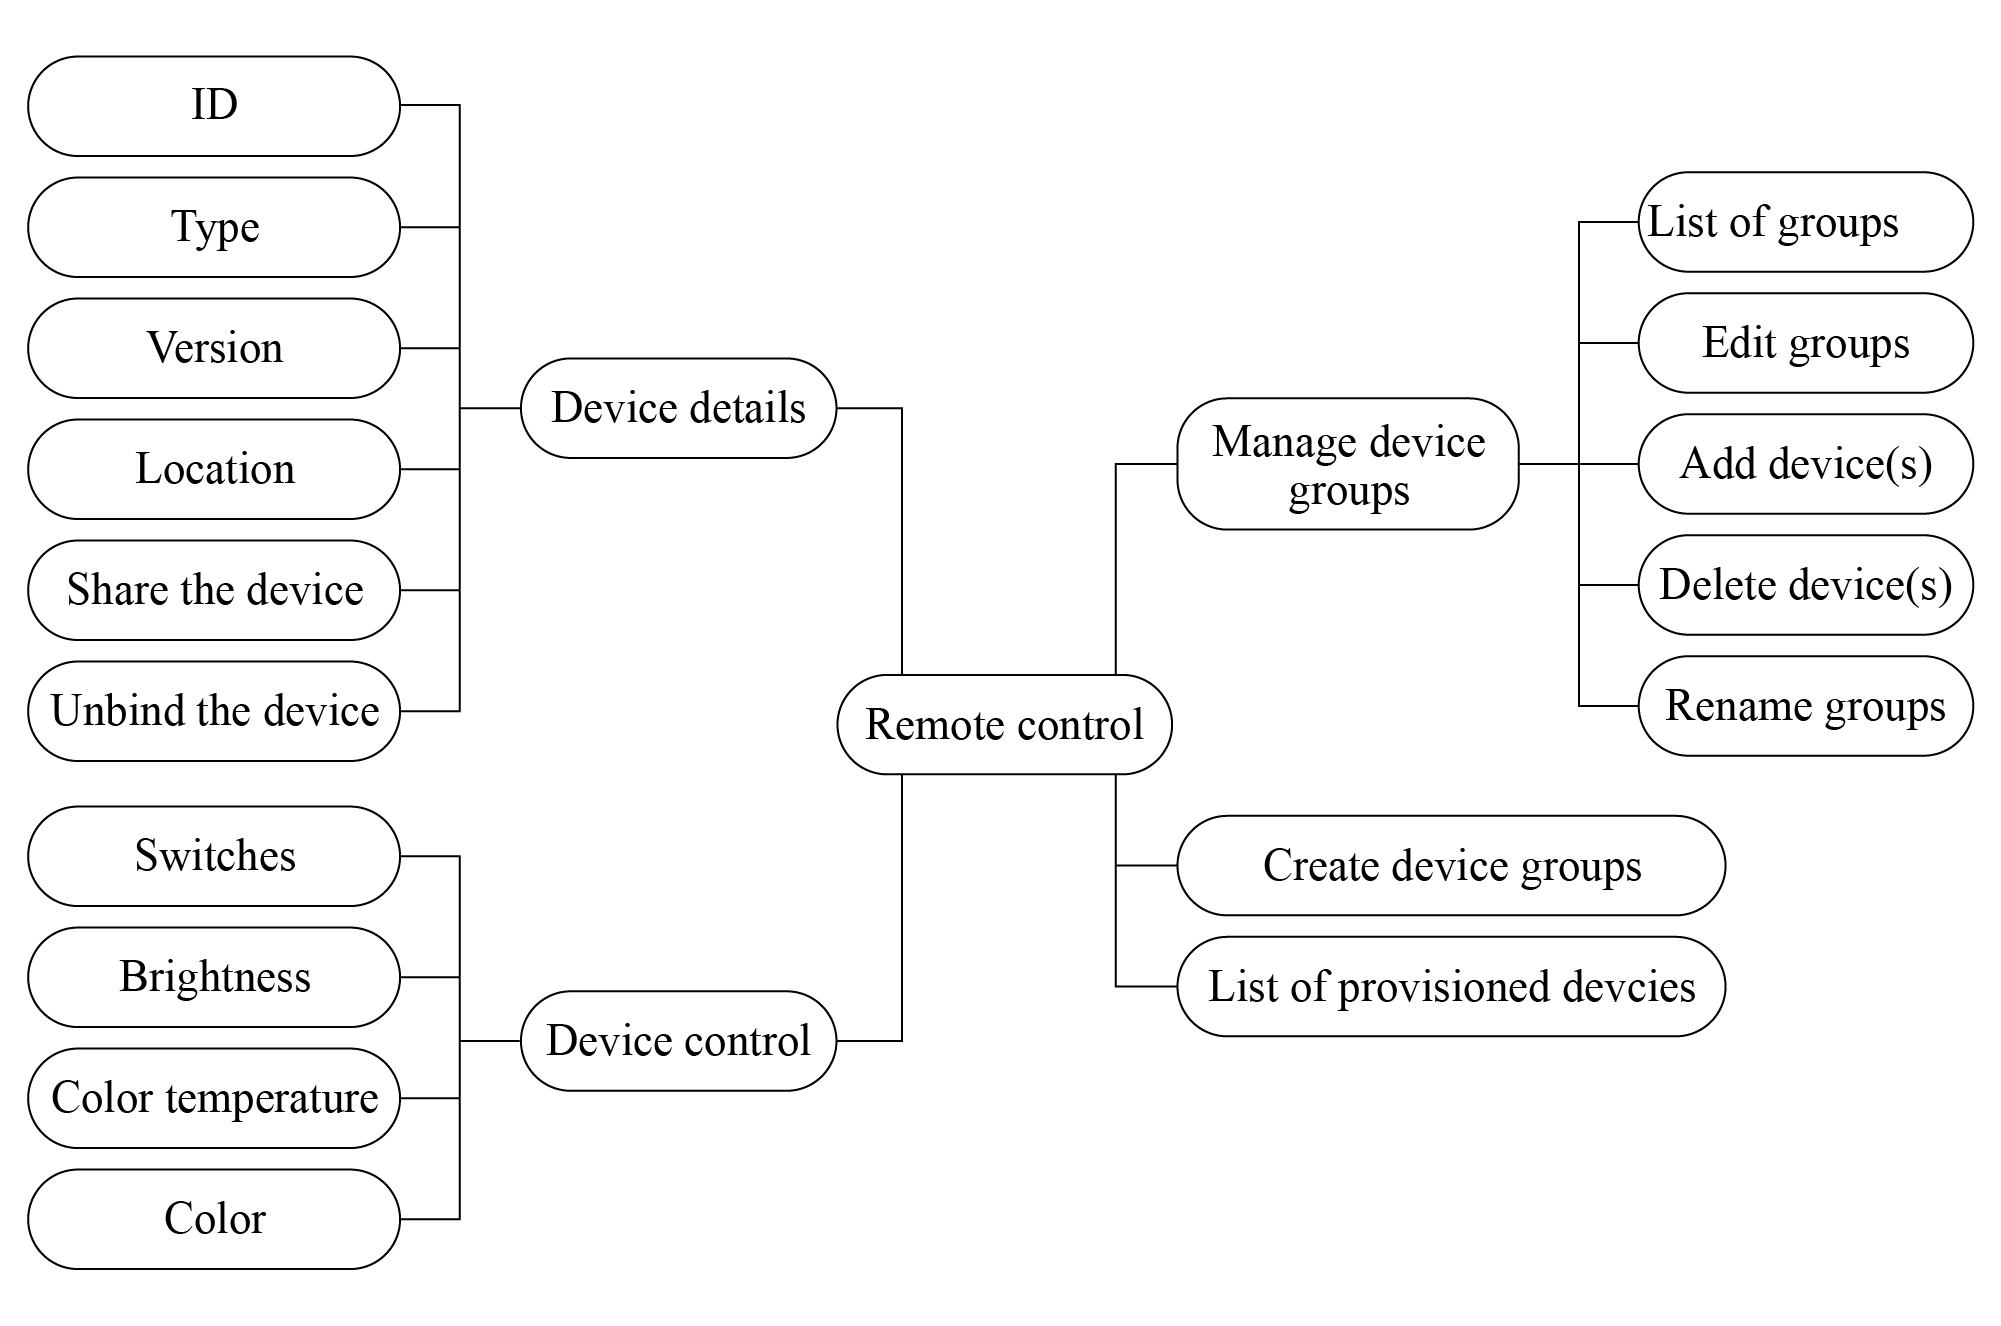
\includegraphics[width=0.65\textwidth]{D10Z/10-15}
    \caption{Analysis of remote-control requirements}
\end{figure}

\begin{itemize}
    \item In the smartphone app, all the provisioned devices will be displayed in a list and can be turned on/off easily.
    \item By selecting a specified device, users will enter its independent control interface, which varies for each device type. For example, it might be used to control switches, brightness, and color.
    \item The device details interface will show device ID, type, version, location, etc., and allow users to analyze and unbind devices.
    \item By creating groups, devices can be controlled and managed together.
\end{itemize}

\subsection{Analysis of Scheduling Requirements}
\begin{figure}[ht]
    \centering
    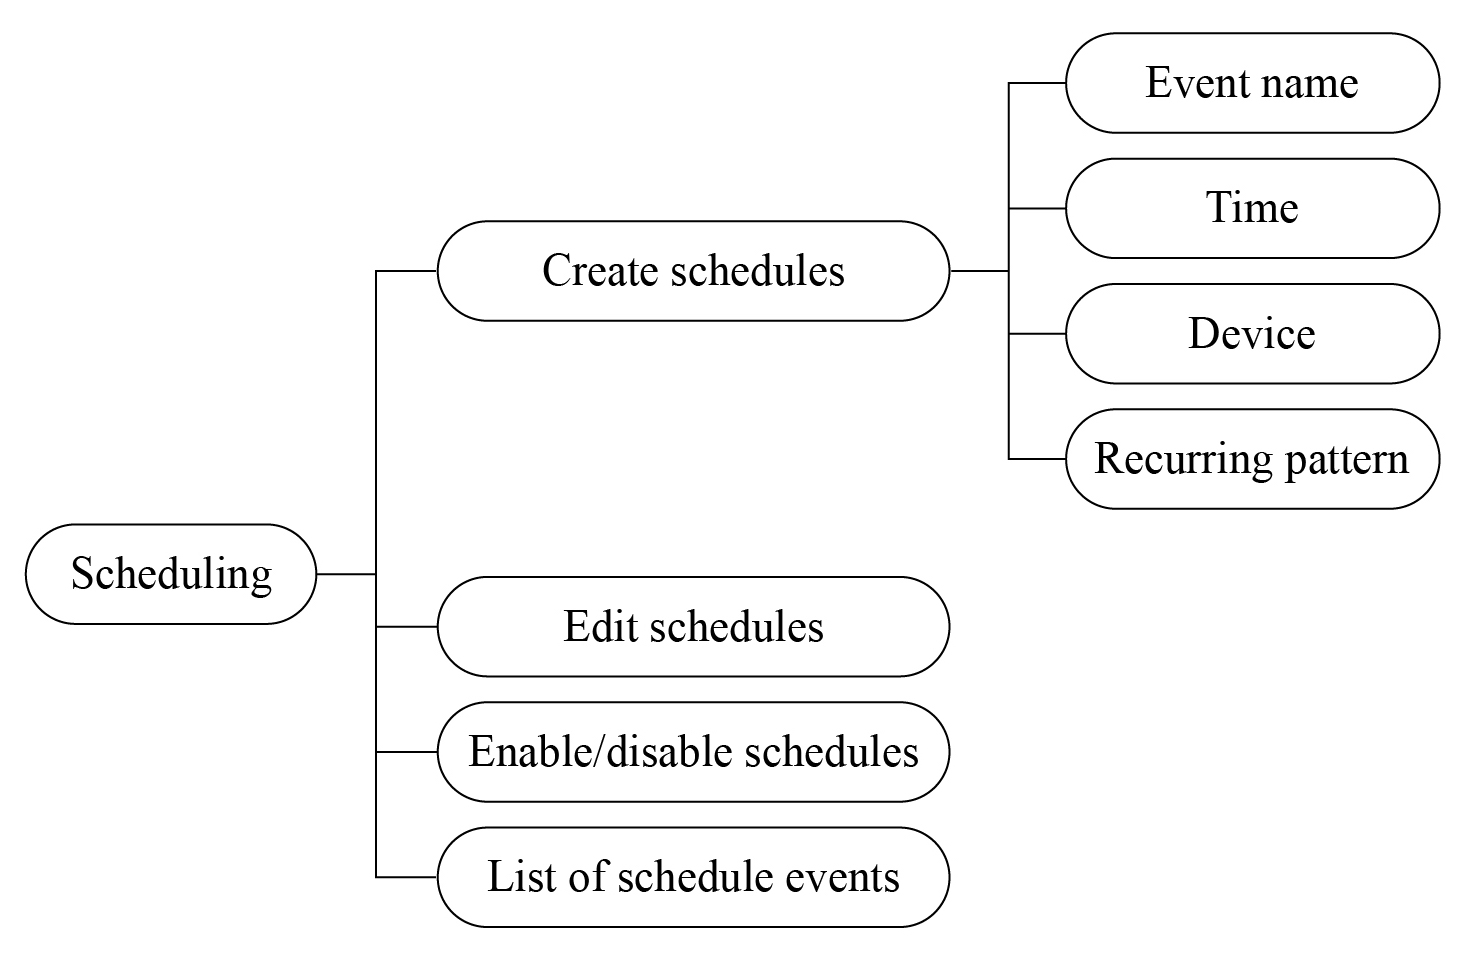
\includegraphics[width=0.6\textwidth]{D10Z/10-16}
    \caption{Analysis of scheduling requirements}
\end{figure}

The scheduling function is relatively simple, very similar to alarm clocks we use every day. It mainly includes functions like creating schedules, list of schedule events, editing schedules, enabling/disabling schedules, etc. The analysis of scheduling requirements is shown in Figure 10.16. The details of a schedule refer to its event name, date, time, recurring pattern, etc.

\subsection{Analysis of User Centre Requirements}
The user centre module mainly features user profile, notification, changing password, terms of use, project documents, privacy policy, voice services, and logout. Note that the changing password and logout functions need to call the cloud API. The analysis of user centre requirements is shown in Figure 10.17.

\begin{figure}[ht]
    \centering
    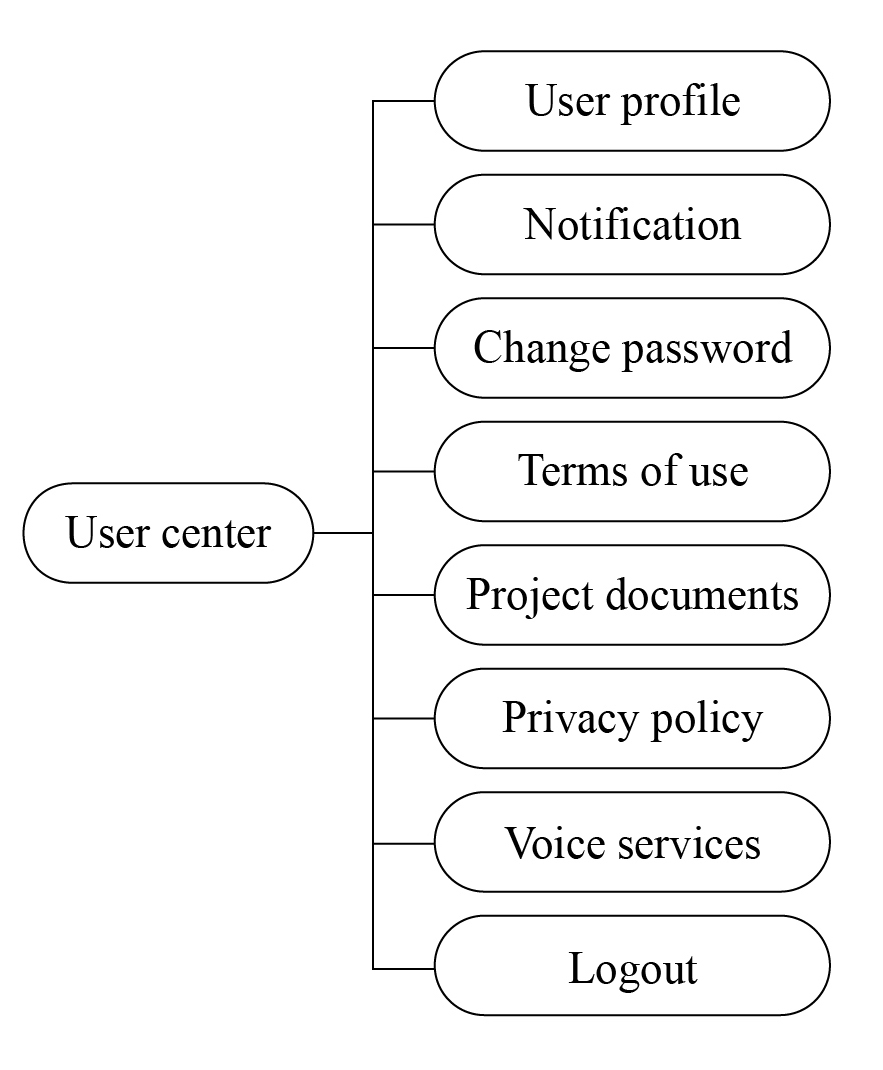
\includegraphics[width=0.35\textwidth]{D10Z/10-17}
    \caption{Analysis of user centre requirements}
\end{figure}

\section{Development of User Management}
After going through the analysis of the project’s functional requirements in Section 10.3, you should already have an overall picture of modules and functions that need to be developed, as well as the required frameworks and third-party libraries. In this section, we will put all the modules and functions into code. Based on the new projects and permissions configured before, now you need to know the classes designed for each interface and associations between them, in order to achieve better operation through code. The code for each function would be encapsulated to be reused and modularised.

\subsection{Introduction to RainMaker APIs}
RainMaker cloud supports two types of APIs: \verb|Unauthenticated| and \verb|Authenticated|. Unauthenticated APIs do not have any authentication tokens in the HTTP header and will receive \verb|access_token| in the response when users log in successfully. Authenticated APIs are marked in the \verb|Swagger| file with a “lock” sign in the front. Their \verb|access_token| needs to be passed for authentification in the \verb|Authorization| HTTP header.

For RainMaker API documentation, please refer to \url{https://swaggerapis.rainmaker.espressif.com}.

When smartphones communicate with the RainMaker cloud, the underlying protocol is HyperText Transfer Protocol Secure (HTTPS). HTTPS can authenticate the server to protect the privacy and integrity of the exchange data. The HTTPS body received by the RainMaker cloud is in JSON format.

\subsection{Initiating Communication via Smartphone}
Android and iOS provide good native support for HTTPS and JSON.

\begin{itemize}
    \item The Android system uses JSONObject and JSONArray to assemble and parse JSON objects and arrays, and HttpURLConnection to initiate HTTPS requests.
    \item The iOS system uses NSJSONSerialization to assemble and parse JSON data, and URLSession to initiate HTTPS requests.
\end{itemize}

Of course, you can also use third-party HTTPS and JSON libraries.

\subsection{Account Registration}
First, we need to implement the registration of a new account, which will be used to bind the device in subsequent steps and control it remotely. In this project, the account is registered via email address.

\begin{figure}[ht]
    \centering
    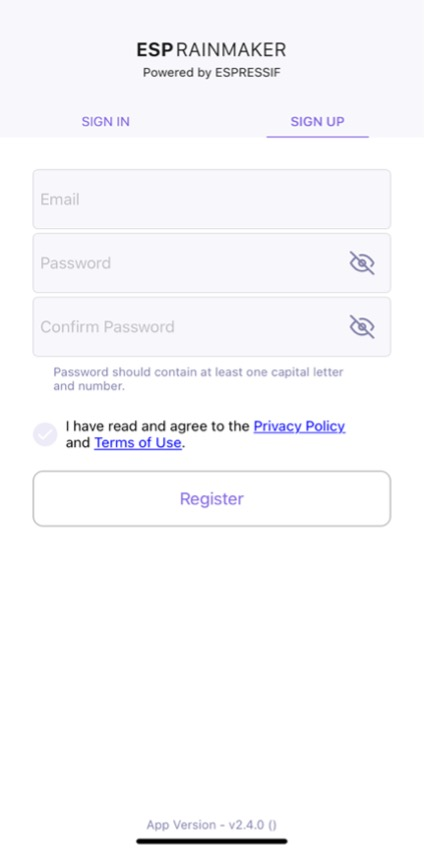
\includegraphics[width=0.25\textwidth,frame]{D10Z/10-18}
    \caption{SIGN UP interface}
\end{figure}

There is a toggle button in the registration interface to switch between “SIGN IN” and “SIGN UP”. For the SIGN UP interface, there are three input fields: Email, Password, and Confirm Password. The content of the Password and Confirm Password fields can be shown or hidden by toggling their visibility, so that users can check whether they have entered the correct password. The password should contain at least one uppercase letter and a number.

Before clicking “Register”, users must read and agree to the Privacy Policy and Terms of Use. Then, it will navigate to a verification interface, and a digital code will be sent to the email address. Users need to enter the correct digital code to complete the registration procedure. The SIGN UP interface is shown in Figure 10.18.

Figure 10.19 demonstrates the API for account registraion. For detailed information, please refer to \url{https://swaggerapis.rainmaker.espressif.com/\#/User/usercreation}.

\begin{figure}[ht]
    \centering
    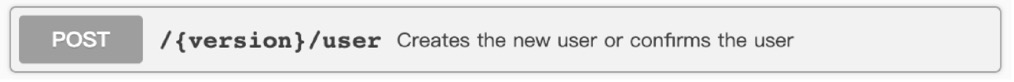
\includegraphics[width=0.9\textwidth]{D10Z/10-19}
    \caption{API for account registration}
\end{figure}

The account registration function is implemented as follows:

\textbf{Create a new account.} Below shows the account registration API, where \verb|user_name| refers to the email address used for registration, and \verb|password| to the password.

\begin{codebloc}
\begin{tabular}{d}
\vspace{2pt}
\begin{verbatim}
1.  POST /v1/user
2.  Content-Type: application/json
3.	
4.  {
5.      "user_name": "username@domain.com",
6.      "password": "password"
\end{verbatim}
\verb|7.  }|
\end{tabular}
\end{codebloc}

To create a new account in Android, use:

\begin{codebloc}
\begin{tabular}{d}
\verb|1.  @POST|\newline
\verb|2.  Call<ResponseBody> createUser(@Url String url, @Body JsonObject body);|
\end{tabular}
\end{codebloc}

\note[Source code]{For the source code of creating a new account in Android, please refer to \href{https://github.com/espressif/book-esp32c3-iot-projects/blob/main/phone_app/app_android/app/src/main/java/com/espressif/cloudapi/ApiInterface.java}{\texttt{book-esp32c3-iot-projects/phone\_app/app\_android/app/src/main/java/\newline com/espressif/cloudapi/ApiInterface.java}}.}

To create a new account in iOS, use:

\begin{codebloc}
\begin{tabular}{d}
\vspace{2pt}
\begin{verbatim}
1.  func createNewUser(name: String, password: String) {
2.    apiWorker.callAPI(endPoint: .createNewUser(url: self.url, name: name,
3.      password: password), encoding: JSONEncoding.default) { data, error in
4.     self.apiParser.parseResponse(data, withError: error) { umError in
5.      self.presenter?.verifyUser(withName: name, andPassword:
6.
\end{verbatim}
\verb|7.  }|
\end{tabular}
\end{codebloc}

%\begin{}

\note[Source code]{For the source code of creating a new account in iOS, please refer to \href{https://github.com/espressif/book-esp32c3-iot-projects/blob/main/phone_app/app_ios/ESPRainMaker/ESPRainMaker/UserManagement/Interactors/ESPCreateUserService.swift}{\texttt{book-esp32c3-\newline iot-projects/phone\_app/app\_ios/ESPRainMaker/ESPRainMaker/\newline UserManagement/Interactors/ESPCreateUserService.swift}}.}

\textbf{Verify the account after receiving the digital code.} Below shows details of the API, where \verb|user_name| refers to the email address used for registration, and \verb|verification_code| to the digital code.

\begin{codebloc}
\begin{tabular}{d}
\vspace{2pt}
\begin{verbatim}
POST /v1/user
Content-Type: application/json

{
    "user_name": "username@domain.com",
    "verification_code": "verification_code"
\end{verbatim}
\verb|}|
\end{tabular}
\end{codebloc}

To verify the account with digital code in Android, use:

\begin{codebloc}
\begin{tabular}{d}
\verb|1.  @POST|\newline
\verb|2.  Call<ResponseBody> confirmUser(@Url String url, @Body JsonObject body);|
\end{tabular}
\end{codebloc}

\note[Source code]{For the source code of verifying the account in Android, please refer to \href{https://github.com/espressif/book-esp32c3-iot-projects/blob/main/phone_app/app_android/app/src/main/java/com/espressif/cloudapi/ApiInterface.java}{\texttt{book-esp32c3-\newline iot-projects/phone\_app/app\_android/app/src/main/java/com/\newline espressif/cloudapi/ApiInterface.java}}.}

To verify the account with digital code in iOS, use:

\begin{codebloc}
\begin{tabular}{d}
\vspace{2pt}
\begin{verbatim}
1.  func confirmUser(name: String, verificationCode: String) {
2.      apiWorker.callAPI(endPoint: .confirmUser(url: self.url, name: name,
3.                          verificationCode: verificationCode),
4.                          encoding: JSONEncoding.default) { data, error in
5.          self.apiParser.parseResponse(data, withError: error) { umError in
6.              self.presenter?.userVerified(withError: umError)
7.          }
8.      }
\end{verbatim}
\verb|9.  }|
\end{tabular}
\end{codebloc}

\note[Source code]{For the source code of verifying the account in iOS, please refer to \href{https://github.com/espressif/book-esp32c3-iot-projects/blob/main/phone_app/app_ios/ESPRainMaker/ESPRainMaker/UserManagement/Interactors/ESPCreateUserService.swift}{\texttt{book-esp32c3-\newline iot-projects/phone\_app/app\_ios/ESPRainMaker/ESPRainMaker/\newline UserManagement/Interactors/ESPCreateUserService.swift}}.}

\subsection{Account Login}
After account registration, we can call the account login API to get the \verb|token| for authentication and the basic profile.

The smartphone app project in this chapter supports login via third-party accounts such as GitHub, Apple, and Google. So long as users have accounts of these three platforms, they can log in directly in the app without registration.

If users have already registered new accounts, they can also log in to the app by entering their email address and password.

If users forget their password, they can click “Forgot password?” under the “Sign in” button to reset password.

At the bottom of the SIGN IN interface are the project-related documentation, privacy agreement, terms of use, and the app version. The SIGN IN interface is shown in Figure 10.20.

\begin{figure}[ht]
    \centering
    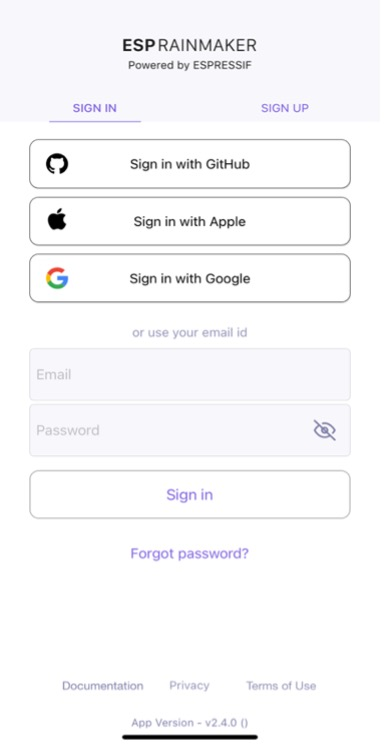
\includegraphics[width=0.32\textwidth,frame]{D10Z/10-20}
    \caption{SIGN IN interface}
\end{figure}

The account login function is implemented as follows:

\textbf{Request an access token.} The API is shown in Figure 10.21 and details can be found at \url{https://swaggerapis.rainmaker.espressif.com/\#/User/login}.

\begin{figure}[ht]
    \centering
    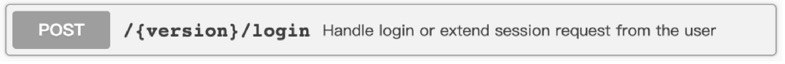
\includegraphics[width=0.8\textwidth]{D10Z/10-21}
    \caption{API for account login}
\end{figure}

\begin{codebloc}
\begin{tabular}{d}
\vspace{2pt}
\begin{verbatim}
POST /v1/login
Content-Type: application/json

{
    "user_name": "username@domain.com",
    "password": "password"
\end{verbatim}
\verb|}|
\end{tabular}
\end{codebloc}

The server responds to the request as follows:

\begin{codebloc}
\begin{tabular}{d}
\vspace{2pt}
\begin{verbatim}
{
    "status": "success",
    "description": "Login successful",
    "idtoken": "idtoken",
    "accesstoken": "accesstoken",
    "refreshtoken": "refreshtoken"
\end{verbatim}
\verb|}|
\end{tabular}
\end{codebloc}

Among these fields, \verb|status| tells whether the request is successful; \verb|description| provides details of the request; \verb|accesstoken| is the token to be added to the HTTP request header by all APIs requiring user permissions, in the format of \verb|Authorization:$acces-|\\
\verb|stoken|; \verb|idtoken| and \verb|refreshtoken| are not used for now and thus not explained here.

To request \verb|access token| in Android, use:

\begin{codebloc}
\begin{tabular}{d}
\verb|1.  @POST|

\verb|2.  Call<ResponseBody> login(@Url String url, @Body JsonObject body);|
\end{tabular}
\end{codebloc}

\note[Source code]{For the source code of requesting access token in Android, please refer to \href{https://github.com/espressif/book-esp32c3-iot-projects/blob/main/phone_app/app_android/app/src/main/java/com/espressif/cloudapi/ApiInterface.java}{\texttt{book-\newline esp32c3-iot-projects/phone\_app/app\_android/app/src/main/java/\newline com/espressif/cloudapi/ApiInterface.java}}.}

To request \verb|access token| in iOS, use:

\begin{codebloc}
\begin{tabular}{d}
\vspace{2pt}
\begin{verbatim}
1.  func loginUser(name: String, password: String) {
2.      apiWorker.callAPI(endPoint: .loginUser(url: self.url,
3.                      name: name, password: password),
4.                      encoding: JSONEncoding.default) { data, error in|
5.          self.apiParser.parseExtendSessionResponse(data,
6.                                          error: error) { _, umError in
7.              self.presenter?.loginCompleted(withError: umError)
8.          }
9.      }
\end{verbatim}
\verb|10. }|
\end{tabular}
\end{codebloc}

\note[Source code]{For the source code of requesting access token in iOS, please refer to \href{https://github.com/espressif/book-esp32c3-iot-projects/blob/main/phone_app/app_ios/ESPRainMaker/ESPRainMaker/UserManagement/Interactors/ESPLoginService.swift}{\texttt{book-esp32c3-\newline iot-projects/phone\_app/app\_ios/ESPRainMaker/ESPRainMaker/\newline UserManagement/Interactors/ESPLoginService.swift}}.}

\vspace{6pt}
\textbf{Get user profile.} The API is shown in Figure 10.22 and details can be found at \url{https://swaggerapis.rainmaker.espressif.com/\#/User/getUser}.

\begin{figure}[ht]
    \centering
    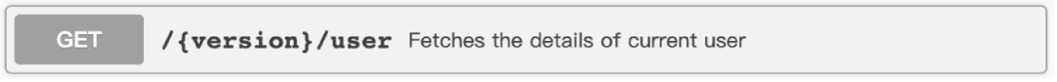
\includegraphics[width=0.68\textwidth]{D10Z/10-22}
    \caption{API to get user profile}
\end{figure}

\begin{codebloc}
\begin{tabular}{d}
\verb|GET /v1/user|

\verb|Authorization: $accesstoken|
\end{tabular}
\end{codebloc}

In response to the “get user profile” request, the server returns:

\begin{codebloc}
\begin{tabular}{d}
\vspace{2pt}
\begin{verbatim}
{
    "user_id": "string",
    "user_name": "string",
    "super_admin": true,
    "picture_url": "string",
    "name": "string",
    "mfa": true,
    "phone_number": "<+Mobile Number with country code>"
\end{verbatim}
\verb|}|
\end{tabular}
\end{codebloc}

Among these fields, \verb|user_id| is the user’s unique identifier and will be used later in provisioning; \verb|user_name| refers to the account; \verb|super_admin| is returned \verb|true| only when the user is a super admin; \verb|picture_url| points to the user’s profile picture; \verb|phone_number| is the user’s mobile phone number; \verb|name| and \verb|mfa| are not used in this project and thus not explained here.

To get user profile in Android, use:

\begin{codebloc}
\begin{tabular}{d}
\verb|1.  @GET|

\verb|2.  Call<ResponseBody> fetchUserDetails(@Url String url);|
\end{tabular}
\end{codebloc}

\note[Source code]{For the source code of getting user profile in Android, please refer to \href{https://github.com/espressif/book-esp32c3-iot-projects/blob/main/phone_app/app_android/app/src/main/java/com/espressif/cloudapi/ApiInterface.java}{\texttt{book-esp32c3-\newline iot-projects/phone\_app/app\_android/app/src/main/java/com/\newline espressif/cloudapi/ApiInterface.java}}.}

To get user profile in iOS, use:

\begin{codebloc}
\begin{tabular}{d}
\vspace{2pt}
\begin{verbatim}
1.  func fetchUserDetails() {
2.    sessionWorker.checkUserSession { accessToken, error in
3.      if let token = accessToken, token.count > 0 {
4.        self.apiWorker.callAPI(endPoint: .fetchUserDetails(url: self.url,
5.                                  accessToken: token), encoding:
6.                                  JSONEncoding.default) { data, error in
7.          self.apiParser.parseUserDetailsResponse(data,
8.                                  withError: error) { umError in
9.            self.presenter?.userDetailsFetched(error: umError)
10.           return
11.         }
12.       }
13.     } else {
14.       self.presenter?.userDetailsFetched(error: error)
15.     }
16.   }
\end{verbatim}
\verb|17. }|
\end{tabular}
\end{codebloc}

\note[Source code]{For the source code of getting user profile in iOS, please refer to \href{https://github.com/espressif/book-esp32c3-iot-projects/blob/main/phone_app/app_ios/ESPRainMaker/ESPRainMaker/UserManagement/Interactors/ESPUserService.swift}{\texttt{book-esp32c3-\newline iot-projects/phone\_app/app\_ios/ESPRainMaker/ESPRainMaker/\newline UserManagement/Interactors/ESPUserService.swift}}.}

\section{Development of Device Provisioning}
As described in Section 10.4, we can get \verb|access token| and \verb|user_id| of the RainMaker account through APIs for account login and getting user profile. The next step is to find the device, connect it to the router, and activitate it on the cloud. The suitable provisioning library for the app is \verb|idf-provisioning|, which is encapsulated based on ESP-IDF provisioning.

For provisioning methods, please refer to \url{https://bookc3.espressif.com/provisioning}.

Figure 10.23 illustrates the data exchange between the smartphone and the device during provisioning. This is also mentioned in Section 7.3.4 Bluetooth Provisioning.

\begin{figure}[ht]
    \centering
    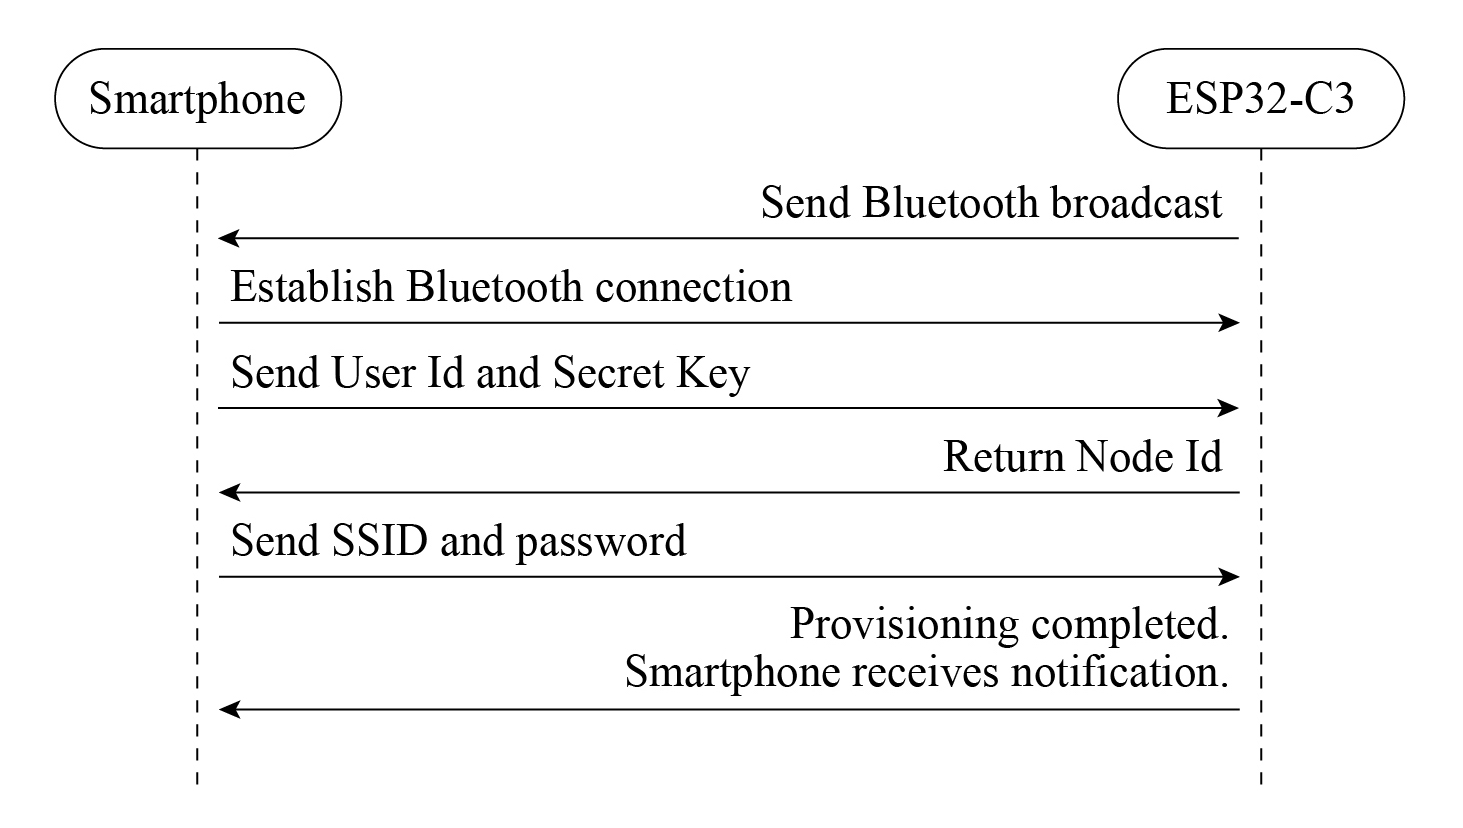
\includegraphics[width=0.8\textwidth]{D10Z/10-23}
    \caption{Data exchange between smartphone and device during provisioning}
\end{figure}

\subsection{Scanning Devices}
Navigate to the homepage of the app, click the button in the upper right corner, and the camera will be called to scan QR Code on devices. This is the fastest way to discover a smart device. Except for QR code scanning, users can also discover devices through BLE or SoftAP provisioning. The device scanning interface is shown in Figure 10.24. (The actual interface may be different from the screenshots in this book due to application upgrades.)

\begin{figure}[ht]
    \centering
    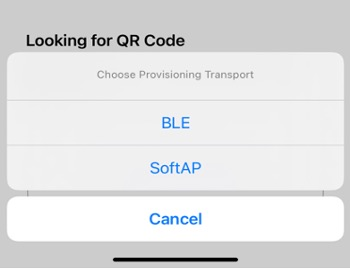
\includegraphics[width=0.55\textwidth]{D10Z/10-24}
    \caption{Device scanning interface}
\end{figure}

In the following sections, we will take Bluetooth provisioning as an example to introduce the process of device provisoning.

\textbf{Scanning devices in Android}

Users should upgrade their phones to Android 9.0 or higher and enable GPS to search for Bluetooth LE signals. The code is as follows:

\note[Source code]{For the source code of scanning devices in Android, please refer to \href{https://github.com/espressif/book-esp32c3-iot-projects/blob/main/phone_app/app_android/app/src/main/java/com/espressif/ui/activities/BLEProvisionLanding.java}{\texttt{book-esp32c3-iot-\newline projects/phone\_app/app\_android/app/src/main/java/com/espressif/ui/\newline activites/BLEProvisionLanding.java}}.}

\vspace{6pt}
\begin{codebloc}
\begin{tabular}{d}
\vspace{2pt}
\begin{verbatim}
1. private void startScan() {
2.  //Code Omitted
3.  if (ActivityCompat.checkSelfPermission(this,
4.                          Manifest.permission.ACCESS_ FINE_LOCATION) ==
5.                          PackageManager.PERMISSION_GRANTED) {
6.    provisionManager.searchBleEspDevices(deviceNamePrefix, bleScanListener);
7.    updateProgressAndScanBtn();
8.  } else {
9.    //Code Omitted
10. }
11.}
12.
13.private BleScanListener bleScanListener = new BleScanListener() {
14. @Override
15. public void scanStartFailed() {
16.    Toast.makeText(BLEProvisionLanding.this,
17.                     "Please turn on Bluetooth to connect BLE device",
18.                     Toast.LENGTH_SHORT).show();
19. }
20.
21. @Override
22. public void onPeripheralFound(BluetoothDevice device,
23.                                             ScanResult scanResult) {
24.    //Code Omitted
25. }
26.
27. @Override
28. public void scanCompleted() {
29.    //Code Omitted
30. }
31.
32. @Override
33. public void onFailure(Exception e) {
34.    //Code Omitted
35. }
\end{verbatim}
\verb|36.};|
\end{tabular}
\end{codebloc}

\textbf{Scanning devices in iOS}

In the following code, \verb|prefix| is used to filter devices by names. If a device has its unique identifier, it can be used for filtering. iOS code has an additional parameter \verb|transport| with two possible values: \verb|ble| and \verb|softap|, which refers to the two provisioning methods.

\note[Source code]{For the source code of scanning devices in iOS, please refer to \href{https://github.com/espressif/book-esp32c3-iot-projects/blob/main/phone_app/app_ios/ESPRainMaker/ESPRainMaker/Interface/Provision/BLE/BLELandingViewController.swift}{\texttt{book-esp32c3-iot-\newline projects/phone\_app/app\_ios/ESPRainMaker/ESPRainMaker/Interface/\newline Provision/BLE/BLELandingViewController.swift}}.}

\begin{codebloc}
\begin{tabular}{d}
\vspace{2pt}
\begin{verbatim}
1.ESPProvisionManager.shared.searchESPDevices(devicePrefix: "prefix",
2. transport: .ble, security:Configuration.shared.espProvSetting.securityMode)
3. { bleDevices, _ in
4.  //Code Omitted
\end{verbatim}
\verb|5.}|
\end{tabular}
\end{codebloc}

\subsection{Connecting Devices}
\textbf{Connecting devices in Android}

\note[Source code]{For the source code of connecting devices in Android, please refer to \href{https://github.com/espressif/book-esp32c3-iot-projects/blob/main/phone_app/app_android/app/src/main/java/com/espressif/ui/activities/BLEProvisionLanding.java}{\texttt{book-esp32c3-\newline iot-projects/phone\_app/app\_android/app/src/main/java/com/\newline espressif/ui/activites/BLEProvisionLanding.java}}.}

\begin{codebloc}
\begin{tabular}{d}
\vspace{2pt}
\begin{verbatim}
1.  override fun onCreate(savedInstanceState: Bundle?) {
2.      super.onCreate(savedInstanceState)
3.      //Code Omitted
4.      EventBus.getDefault().register(this)
5.  }
6.
7.  @Override
8.  protected void onDestroy() {
9.      EventBus.getDefault().unregister(this);
10.     super.onDestroy();
11. }
12.
13. @Subscribe(threadMode = ThreadMode.MAIN)
14. public void onEvent(DeviceConnectionEvent event) {
15.     handler.removeCallbacks(disconnectDeviceTask);
16.     switch (event.getEventType()) {
17.         case ESPConstants.EVENT_DEVICE_CONNECTED:
18.         //Code Omitted
19.         break;
20.
\end{verbatim}
\verb|21.         case ESPConstants.EVENT_DEVICE_DISCONNECTED:|
\end{tabular}
\end{codebloc}

\begin{codebloc}
\begin{tabular}{d}
\vspace{2pt}
\begin{verbatim}
22.         //Code Omitted
23.         break;
24.
25.         case ESPConstants.EVENT_DEVICE_CONNECTION_FAILED:
26.         //Code Omitted
27.         break;
28.     }
\end{verbatim}
\verb|29. }|
\end{tabular}
\end{codebloc}

In Android, EventBus is used to notify activities when Bluetooth LE connection status changes, so it is necessary to register a callback function in activities. After the device has been discovered, we should first create a device instance as shown in the code above, and then call the connection API as follows, so that the smartphone app can initiate a connection request to the device.

\begin{codebloc}
\begin{tabular}{d}
\vspace{2pt}
\begin{verbatim}
1.  public void deviceClick(int deviceClickedPosition) {
2.    stopScan();
3.    isConnecting = true;
4.    isDeviceConnected = false;
5.    btnScan.setVisibility(View.GONE);
6.    rvBleDevices.setVisibility(View.GONE);
7.    progressBar.setVisibility(View.VISIBLE);
8.    this.position = deviceClickedPosition;
9.    BleDevice bleDevice = deviceList.get(deviceClickedPosition);
10.   String uuid = bluetoothDevices.get(bleDevice.getBluetoothDevice());
11.
12.   if (ActivityCompat.checkSelfPermission(BLEProvisionLanding.this,
13.                         Manifest. permission.ACCESS_FINE_LOCATION) ==
14.                         PackageManager.PERMISSION_GRANTED) {
15.     boolean isSec1 = true;
16.     if (AppConstants.SECURITY_0.equalsIgnoreCase(BuildConfig.SECURITY)) {
17.         isSec1 = false;
18.     }
19.     if (isSec1) {
20.       provisionManager.createESPDevice(ESPConstants.TransportType.
21.           TRANSPORT_BLE, ESPConstants.SecurityType.SECURITY_1);
22.     } else {
23.       provisionManager.createESPDevice(ESPConstants.TransportType.
24.                   TRANSPORT_BLE, ESPConstants.SecurityType.SECURITY_0);
25.     }provisionManager.getEspDevice().connectBLEDevice(bleDevice.
26.                                         getBluetoothDevice(), uuid);
27.     handler.postDelayed(disconnectDeviceTask, DEVICE_CONNECT_TIMEOUT);
28.   } else {
29.     Log.e(TAG, "Not able to connect device as Location permission is
30.                                                         not granted." );
31.   }
\end{verbatim}
\verb|32. }|
\end{tabular}
\end{codebloc}

\note[Source code]{For the source code of initiating a connection by the smartphone app, please refer to \href{https://github.com/espressif/book-esp32c3-iot-projects/blob/main/phone_app/app_android/app/src/main/java/com/espressif/ui/activities/BLEProvisionLanding.java}{\texttt{book-esp32c3-iot-projects/phone\_app/app\_android/app/src/main/java/\newline com/espressif/ui/activites/BLEProvisionLanding.java}}.}

\textbf{Connecting devices in iOS}

The iOS app provides a proxy for the connection callback function, so we can directly call the instance connection interface returned by device scanning and pass the status proxy as a parameter to \verb|bleConnectionStatusHandler|. The code is as follows:

\note[Source code]{The \texttt{pods} folder stores imported third-party libraries. Files in this folder will only be generated once the project is compiled and installed locally. For the source code of connecting devices in iOS, please refer to \texttt{book-esp32c3-iot-projects/phone\_\newline app/pods/espprovision/ESPDevice.swift}.}

\begin{codebloc}
\begin{tabular}{d}
\vspace{2pt}
\begin{verbatim}
1.  open func connect(delegate: ESPDeviceConnectionDelegate? = nil,
2.              completionHandler: @escaping (ESPSessionStatus) -> Void) {
3.      ESPLog.log("Connecting ESPDevice..." )
4.      self.delegate = delegate
5.      switch transport {
6.          case .ble:
7.              ESPLog.log("Start connecting ble device." )
8.              bleConnectionStatusHandler = completionHandler
9.              if espBleTransport == nil {
10.                 espBleTransport = ESPBleTransport(scanTimeout: 0,
11.                                                 deviceNamePrefix: "")
12.             }
13.             espBleTransport.connect(peripheral: peripheral, 
14.                                     withOptions:
15.                                     nil, 
16.                                     delegate: self) 
17.         case .softap:
18.             ESPLog.log("Start connecting SoftAp device." )
19.             if espSoftApTransport == nil {
20.                 espSoftApTransport = ESPSoftAPTransport(baseUrl:
21.                                                     ESPUtility.baseUrl)
22.             }
23.             self.connectToSoftApUsingCredentials(ssid: name,
24.                                 completionHandler: completionHandler)
25.     }
\end{verbatim}
\verb|26. }|
\end{tabular}
\end{codebloc}

\subsection{Generating Secret Keys}
Secret keys are used for authentication when users bind devices, and can be randomly generated by the smartphone app. To generate a secret key in Android, add:

\begin{codebloc}
\begin{tabular}{d}
\verb|1.  final String secretKey = UUID.randomUUID().toString();|
\end{tabular}
\end{codebloc}

To generate a secret key in iOS, add:

\begin{codebloc}
\begin{tabular}{d}
\verb|1.  let secretKey = UUID().uuidString|
\end{tabular}
\end{codebloc}

\subsection{Getting Node ID}
Each device has its unique identifier, namely the node ID. After the device is provisioned, it can be bound to the cloud server via its node ID by calling a binding request. The purpose of binding is to ensure subsequent remote control.

\textbf{Getting Node ID in Android}

\note[Source code]{For the source code of getting node ID in Android, please refer to \href{https://github.com/espressif/book-esp32c3-iot-projects/blob/main/phone_app/app_android/app/src/main/java/com/espressif/ui/activities/ProvisionActivity.java}{\texttt{book-esp32c3-iot-\newline projects/phone\_app/app\_android/app/src/main/java/com/espressif/ui/\newline activites/ProvisionActivity.java}}.}

To create the request for node ID, use:

\begin{codebloc}
\begin{tabular}{d}
\vspace{2pt}
\begin{verbatim}
1.  EspRmakerUserMapping.CmdSetUserMapping deviceSecretRequest =
2.  EspRmakerUser Mapping.CmdSetUserMapping.newBuilder()
3.                      .setUserID(ApiManager.userId)
4.                      .setSecretKey(secretKey)
5.                      .build();
6.  EspRmakerUserMapping.RMakerConfigMsgType msgType =EspRmakerUserMapping.
7.                      RMakerConfigMsgType.TypeCmdSetUserMapping;
8.  EspRmakerUserMapping.RMakerConfigPayload payload = EspRmakerUserMapping.
9.                      RMakerConfigPayload.newBuilder()
10.                     .setMsg(msgType)
11.                     .setCmdSetUserMapping(deviceSecretRequest)
\end{verbatim}
\verb|12.                     .build();|
\end{tabular}
\end{codebloc}

To initiate the request, use:

\begin{codebloc}
\begin{tabular}{d}
\vspace{2pt}
\begin{verbatim}
1.  private void associateDevice() {
2.   provisionManager.getEspDevice().sendDataToCustomEndPoint(AppConstants.
3.   HANDLER_RM_USER_MAPPING, payload.toByteArray(), new ResponseListener() {
4.          @Override
5.          public void onSuccess(byte[] returnData) {
6.              processDetails(returnData, secretKey);
7.          }
8.          @Override
\end{verbatim}
\verb|9.          public void onFailure(Exception e) {|
\end{tabular}
\end{codebloc}

\begin{codebloc}
\begin{tabular}{d}
\vspace{2pt}
\begin{verbatim}
10.             //Code Omitted
11.         }
12.  });
\end{verbatim}
\verb|13.  }|
\end{tabular}
\end{codebloc}

To parse the device’s response, use:

\begin{codebloc}
\begin{tabular}{d}
\vspace{2pt}
\begin{verbatim}
1. private void processDetails(byte[] responseData, String secretKey) {
2.
3.  try {
4.   EspRmakerUserMapping.RMakerConfigPayload payload = EspRmakerUserMapping.
5.                          RMakerConfigPayload.parseFrom(responseData);
6.   EspRmakerUserMapping.RespSetUserMapping response = payload.
7.                                    getRespSetUserMapping();
8.	
9.   if (response.getStatus() == EspRmakerUserMapping.RMakerConfigStatus.
10.                                         Success) {
11.             //Node ID received. Ready for device provisioning.
12.    receivedNodeId = response.getNodeId();
13.   }
14.  } catch (InvalidProtocolBufferException e) {
15.         //Code Omitted
16.  }
\end{verbatim}
\verb|17.}|
\end{tabular}
\end{codebloc}

\textbf{Getting Node ID in iOS}

\note[Source code]{For the source code of getting node ID in iOS, please refer to \href{https://github.com/espressif/book-esp32c3-iot-projects/blob/cf25c67fbcedc44394fd7f90637b745d659f80ff/phone_app/app_ios/ESPRainMaker/ESPRainMaker/AWSCognito/DeviceAssociation.swift}{\texttt{book-esp32c3-iot-\newline projects/phone\_app/app\_ios/ESPRainMaker/ESPRainMaker/AWSCognito/\newline DeviceAssociation.swift}}.}

\begin{codebloc}
\begin{tabular}{d}
\vspace{2pt}
\begin{verbatim}
1.  private func createAssociationConfigRequest() throws -> Data? {
2.      var configRequest = Rainmaker_CmdSetUserMapping()
3.      configRequest.secretKey = secretKey
4.      configRequest.userID = User.shared.userInfo.userID
5.      var payload = Rainmaker_RMakerConfigPayload()
6.      payload.msg = Rainmaker_RMakerConfigMsgType.typeCmdSetUserMapping
7.      payload.cmdSetUserMapping = configRequest
8.      return try payload.serializedData()
\end{verbatim}
\verb|9.  }|
\end{tabular}
\end{codebloc}

To initiate the request, use:

\begin{codebloc}
\begin{tabular}{d}
\vspace{2pt}
\begin{verbatim}
1.  func associateDeviceWithUser() {
2.      do {
3.          let payloadData = try createAssociationConfigRequest()
4.          if let data = payloadData {
5.              device.sendData(path: Constants.associationPath, data: data)
\end{verbatim}
\verb|6.                                                  { response, error in|
\end{tabular}
\end{codebloc}

\begin{codebloc}
\begin{tabular}{d}
\vspace{2pt}
\begin{verbatim}
7.                  guard error == nil, response ! = nil else {
8.                      self.delegate?.deviceAssociationFinishedWith(success:
9.                                  false, nodeID: nil,
10.                                 error: AssociationError.runtimeError
11.                                 (error!.localizedDescription))
12.                     return
13.                 }
14.                 self.processResponse(responseData: response!)
15.             }
16.         } else {
17.           delegate?.deviceAssociationFinishedWith(success: false, nodeID:
18.                             nil, error: AssociationError.runtimeError
19.                             ("Unable to fetch request payload." ))
20.         }
21.     } catch {
22.      delegate?.deviceAssociationFinishedWith(success: false, nodeID: nil,
23.                                 error: AssociationError.runtimeError
24.                                 ("Unable to fetch request payload." ))
25.     }
\end{verbatim}
\verb|26. }|
\end{tabular}
\end{codebloc}

To parse the device’s response, use:

\begin{codebloc}
\begin{tabular}{d}
\vspace{2pt}
\begin{verbatim}
1.  func processResponse(responseData: Data) {
2.      do {
3.          let response = try Rainmaker_RMakerConfigPayload(serializedData:
4.                                                          response Data)
5.          if response.respSetUserMapping.status == .success {
6.              //Node ID received. Ready for device provisioning.
7.          delegate?.deviceAssociationFinishedWith(success: true, nodeID:
8.                      response. respSetUserMapping.nodeID, error: nil)
9.          } else {
10.         delegate?.deviceAssociationFinishedWith(success: false, nodeID:
11.                             nil, error: AssociationError.runtimeError
12.                             ("User node mapping failed." ))
13.         }
14.     } catch {
15.     delegate?.deviceAssociationFinishedWith(success: false, nodeID: nil,
16.                             error: AssociationError.runtimeError
17.                             (error.localizedDescription))
18.     }
\end{verbatim}
\verb|19. }|
\end{tabular}
\end{codebloc}

\subsection{Provisioning Devices}
Once the smartphone app establishes a connection with the device, we can implement protocols through Bluetooth communication, provision the device, and activate the device on the cloud. The entire provisioning process consists of five steps as listed in Figure 10.25.

\begin{figure}[ht]
    \centering
    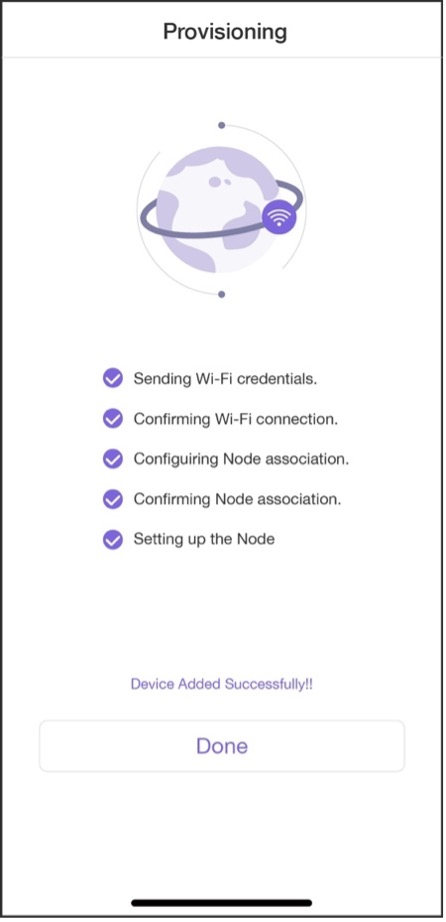
\includegraphics[width=0.35\textwidth]{D10Z/10-25}
    \caption{Device provisioning interface}
\end{figure}

\textbf{Provisioning devices in Android}

\note[Source code]{For the source code of provisioning in Android, please refer to \href{https://github.com/espressif/book-esp32c3-iot-projects/blob/main/phone_app/app_android/app/src/main/java/com/espressif/ui/activities/ProvisionActivity.java}{\texttt{book-esp32c3-iot-\newline projects/phone\_app/app\_android/app/src/main/java/com/espressif/\newline ui/activites/ProvisionActivity.java}}.}

\begin{codebloc}
\begin{tabular}{d}
\vspace{2pt}
\begin{verbatim}
1.  private void provision() {
2.
3.      provisionManager.getEspDevice().provision(ssidValue, passphraseValue,
4.                                              new ProvisionListener() {
5.          @Override
6.          public void createSessionFailed(Exception e) {}
7.          @Override
8.          public void wifiConfigSent() {}
9.          @Override
10.         public void wifiConfigFailed(Exception e) {}
11.         @Override
\end{verbatim}
\verb|12.         public void wifiConfigApplied() {}|
\end{tabular}
\end{codebloc}

\begin{codebloc}
\begin{tabular}{d}
\vspace{2pt}
\begin{verbatim}
13.         @Override
14.         public void wifiConfigApplyFailed(Exception e) {}
15.         @Override
16.         public void provisioningFailedFromDevice(final ESPConstants.
17.                             Provision FailureReason failureReason) {}
18.         @Override
19.         public void deviceProvisioningSuccess() {
20.             // Provisioning succeeded.
21.         }
22.         @Override
23.         public void onProvisioningFailed(Exception e) {}
24.     });
\end{verbatim}
\verb|25. }|
\end{tabular}
\end{codebloc}

\vspace{6pt}
\textbf{Provisioning devices in iOS}

\note[Source code]{For the source code of provisioning in iOS, please refer to \href{https://github.com/espressif/book-esp32c3-iot-projects/blob/cf25c67fbcedc44394fd7f90637b745d659f80ff/phone_app/app_ios/ESPRainMaker/ESPRainMaker/Interface/Provision/SuccessViewController.swift}{\texttt{book-esp32c3-iot-\newline projects/phone\_app/app\_ios/ESPRainMaker/ESPRainMaker/Interface/\newline Provision/SuccessViewController.swift}}.}

\begin{codebloc}
\begin{tabular}{d}
\vspace{2pt}
\begin{verbatim}
1.  espDevice.provision(ssid: ssid, passPhrase: passphrase) { status in
2.      switch status {
3.      case .success:
4.      //Provisioning succeeded.
5.      case let .failure(error):
6.          switch error {
7.              case .configurationError:
8.              case .sessionError:
9.              case .wifiStatusDisconnected:
10.             default:
11.         }
12.     case .configApplied:
13.     }
\end{verbatim}
\verb|14. }|
\end{tabular}
\end{codebloc}

Once the device is provisioned, we are ready to develop the device control function of the smartphone app.

\section{Development of Device Control}
In Section 10.5, we have learned how to provision and activate devices. In this section, we will set about to bind the device to the cloud account and manage to control it.

\subsection{Binding Devices to Cloud Accounts}
API for binding devices to accounts is shown in Figure 10.26 and can be found at \href{https://swaggerapis.rainmaker.espressif.com/#/User%20Node%20Association/addRemoveUserNodeMapping}{https://\newline swaggerapis.rainmaker.espressif.com/\#/User\%20Node\%20Association/addRemoveUser-\newline NodeMapping}.

\begin{figure}[ht]
    \centering
    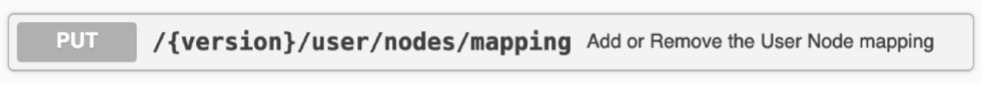
\includegraphics[width=0.8\textwidth]{D10Z/10-26}
    \caption{API for binding devices}
\end{figure}

To bind the device to the account, use the secret key generated in Section 10.5.3, the device ID (\verb|node_id|) and the \verb|operation| identifier.

\begin{codebloc}
\begin{tabular}{d}
\vspace{2pt}
\begin{verbatim}
PUT /v1/user/nodes/mapping
Content-Type: application/json
Authorization: $accesstoken

{
        "node_id": "$node_id",
        "secret_key": "$secretKey",
        "operation": "add"
\end{verbatim}
\verb|}|
\end{tabular}
\end{codebloc}

\vspace{6pt}
\textbf{Binding devices in Android}

\note[Source code]{For the source code of binding devices in Android, please refer to \href{https://github.com/espressif/book-esp32c3-iot-projects/blob/main/phone_app/app_android/app/src/main/java/com/espressif/cloudapi/ApiManager.java}{\texttt{book-esp32c3-iot-\newline projects/phone\_app/app\_android/app/src/main/java/com/espressif/\newline cloudapi/ApiManager.java}}.}

\begin{codebloc}
\begin{tabular}{d}
\vspace{2pt}
\begin{verbatim}
1.  public void addNode(final String nodeId,
2.                      String secretKey,
3.                      final ApiResponseListener listener) {
4.      DeviceOperationRequest req = new DeviceOperationRequest();
5.      req.setNodeId(nodeId);
6.      req.setSecretKey(secretKey);
7.      req.setOperation(AppConstants.KEY_OPERATION_ADD);
8.
9.      apiInterface.addNode(AppConstants.URL_USER_NODE_MAPPING, accessToken,
10.                         req). enqueue(new Callback<ResponseBody>() {
11.
12.         @Override
13.         public void onResponse(Call<ResponseBody> call,
14.                                 Response<ResponseBody> response) {
15.             //Code Omitted
\end{verbatim}
\verb|16.         }|
\end{tabular}
\end{codebloc}

\begin{codebloc}
\begin{tabular}{d}
\vspace{2pt}
\begin{verbatim}
17.         @Override
18.         public void onFailure(Call<ResponseBody> call, Throwable t) {
19.         }
20.     });
\end{verbatim}
\verb|21. }|
\end{tabular}
\end{codebloc}

\vspace{6pt}
\textbf{Binding devices in iOS}

\note[Source code]{For the source code of binding devices in iOS, please refer to \href{https://github.com/espressif/book-esp32c3-iot-projects/blob/cf25c67fbcedc44394fd7f90637b745d659f80ff/phone_app/app_ios/ESPRainMaker/ESPRainMaker/Interface/Provision/SuccessViewController.swift}{\texttt{book-esp32c3-iot-\newline projects/phone\_app/app\_ios/ESPRainMaker/ESPRainMaker/Interface/\newline Provision/SuccessViewController.swift}}.}

\begin{codebloc}
\begin{tabular}{d}
\vspace{2pt}
\begin{verbatim}
1.  @objc func sendRequestToAddDevice() {
2.      let parameters = ["user_id": User.shared.userInfo.userID,
3.                      "node_id":
4.                      User. shared.currentAssociationInfo!.nodeID, 
5.                      "secret_key":User.shared.currentAssociationInfo!.uuid, 
6.                      "operation": "add"]
7.      NetworkManager.shared.addDeviceToUser(parameter: parameters as!
8.                                  [String: String]) { requestID, error in
9.          if error ! = nil, self.count > 0 {
10.             self.count = self.count - 1
11.             DispatchQueue.main.asyncAfter(deadline: .now()) {
12.                 self.perform(#selector(self.sendRequestToAddDevice),
13.                                 with:nil,
14.                                 afterDelay: 5.0)
15.             }
16.         } else {
17.             if let requestid = requestID {
18.                 self.step3Indicator.stopAnimating()
19.                 self.step3Image.image = UIImage(named: "checkbox_checked")
20.                 self.step3Image.isHidden = false
21.                 self.step4ConfirmNodeAssociation(requestID: requestid)
22.             } else {
23.               self.step3FailedWithMessage(message: error?.description ??
24.                     "Unrecognized error. Please check your internet.")
25.             }
26.         }
27.     }
\end{verbatim}
\verb|28. }|
\end{tabular}
\end{codebloc}

Once the device is bound to the account, users can initiate the request for remote communication.

\subsection{Getting a List of Devices}
When users get all the devices bound to the account, the smartphone app would show them in a list. At the top of the interface, there are several toggles for device groups. By default, all the devices will appear in the “All Devices” group. If users want to assign the devices to different groups, they may click the “
\includegraphics[width=0.02\textwidth]{D10Z/dot}” icon on the right and will then see the options to manage and create groups.

\begin{figure}[ht]
    \centering
    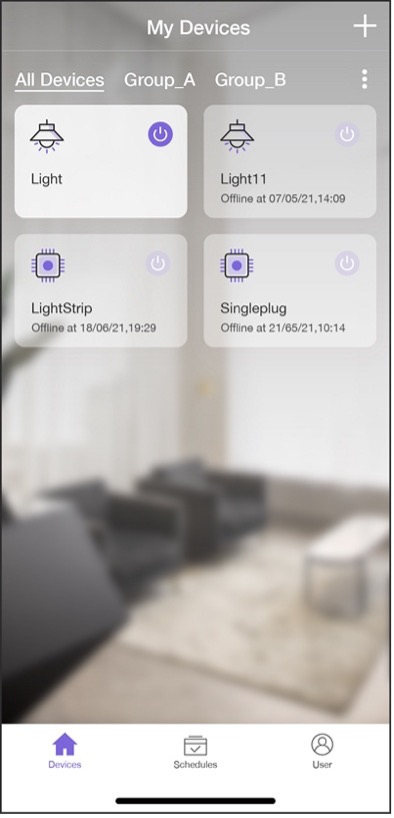
\includegraphics[width=0.33\textwidth]{D10Z/10-27}
    \caption{Interface showing the list of all bound devices}
\end{figure}

Devices grayed out indicate powered down and offline, while devices highlighted indicate available online. The device card includes device type icon, device name, offline time, and a toggle switch. Figure 10.27 shows an example list of all devices bound to the account.

The API to get all the bound devices is shown in Figure 10.28 and can be found at \href{https://swaggerapis.rainmaker.espressif.com/#/User%20Node%20Association/getUserNodeMappingRequestStatus}{https://\newline swaggerapis.rainmaker.espressif.com/\#/User\%20Node\%20Association/getUserNode-\newline MappingRequestStatus}.

\begin{figure}[ht]
    \centering
    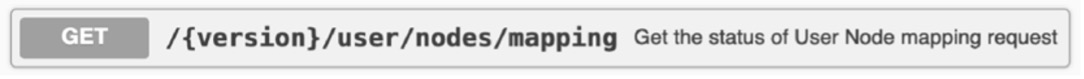
\includegraphics[width=0.8\textwidth]{D10Z/10-28}
    \caption{API to get bound devices}
\end{figure}

\begin{codebloc}
\begin{tabular}{d}
\verb|GET /v1/user/nodes?node_details=true|

\verb|Authorization: $accesstoken|
\end{tabular}
\end{codebloc}

In response to the request, the server returns:

\begin{codebloc}
\begin{tabular}{d}
\vspace{2pt}
\begin{verbatim}
{
        "nodes": "[ nodeid1, ... ]",
        "node_details": [
        {
            "id": "nodeid1",
            "role": "primary",
            "status": {
            "connectivity": {
                    "connected": true,
                    "timestamp": 1584698464101
                }
            },
            "config": {
                "node_id": "nodeid1",
                "config_version": "config_version",
                "devices": [
                {}
                ],
                "info": {
                    "fw_version": "fw_version",
                    "name": "node_name",
                    "type": "node_type"
                }
            },
            "params": {
                "Light": {
                    "brightness": 0,
                    "output": true
                },
                "Switch": {
                    "output": true
                }
            }
        }
        ],
        "next_id": "nodeid1",
        "total": 5
\end{verbatim}
\verb|}|
\end{tabular}
\end{codebloc}

Among these returned fields, \verb|nodes| is an array of all the devices’ ID; \verb|node_details| is the detailed information of the devices, which includes \verb|id| (unique identifier), \verb|role|, \verb|status| (connection status), \verb|config| (configuration), \verb|params| (device properties), etc.; \verb|total| is the number of devices and is returned when device information spread across pages.

\textbf{Getting device information in Android}

\note[Source code]{For the source code of getting device information in Android, please refer to \href{https://github.com/espressif/book-esp32c3-iot-projects/blob/main/phone_app/app_android/app/src/main/java/com/espressif/cloudapi/ApiManager.java}{\texttt{book-\newline esp32c3-iot-projects/phone\_app/app\_android/app/src/main/java/com/\newline espressif/cloudapi/ApiManager.java}}.}

\begin{codebloc}
\begin{tabular}{d}
\vspace{2pt}
\begin{verbatim}
1.  private void getNodesFromCloud(final String startId,
2.                                  final ApiResponseListener listener) {
3.
4.      Log.d(TAG, "Get Nodes from cloud with start id : " + startId);
5.      apiInterface.getNodes(AppConstants.URL_USER_NODES_DETAILS, 
6.                          accessToken,
7.                          startId).enqueue(new Callback<ResponseBody>() {
8.          @Override
9.          public void onResponse(Call<ResponseBody> call,
10.                                 Response<ResponseBody> response) {
11.             //Code Omitted
12.         }
13.         @Override
14.         public void onFailure(Call<ResponseBody> call, Throwable t) {
15.             t.printStackTrace();
16.             listener.onNetworkFailure(new Exception(t));
17.         }
18.     });
\end{verbatim}
\verb|19. }|
\end{tabular}
\end{codebloc}

\vspace{3pt}
\textbf{Getting device information in iOS}

\note[Source code]{For the source code of getting device information in iOS, please refer to \href{https://github.com/espressif/book-esp32c3-iot-projects/blob/cf25c67fbcedc44394fd7f90637b745d659f80ff/phone_app/app_ios/ESPRainMaker/ESPRainMaker/AWSCognito/ESPAPIManager.swift}{\texttt{book-esp32c3-\newline iot-projects/phone\_app/app\_ios/ESPRainMaker/ESPRainMaker/\newline AWSCognito/ESPAPIManager.swift}}.}

\begin{codebloc}
\begin{tabular}{d}
\vspace{2pt}
\begin{verbatim}
1.  func getNodes(partialList: [Node]? = nil, nextNodeID: String? = nil,
2.       completionHandler: @escaping ([Node]?, ESPNetworkError?) -> Void) {
3.      let sessionWorker = ESPExtendUserSessionWorker()
4.      sessionWorker.checkUserSession() { accessToken, error in
5.        if let token = accessToken {
6.          let headers: HTTPHeaders = ["Content-Type": "application/json",
7.                                          "Authorization": token]
8.          var url=Constants.getNodes + "?node_details=true&num_records=10"
9.          if nextNodeID ! = nil {
10.                 url += "&start_id=" + nextNodeID!
11.         }
12.         self.session.request(url, method: .get, 
\end{verbatim}
\verb|13.                             parameters: nil,|
\end{tabular}
\end{codebloc}

\begin{codebloc}
\begin{tabular}{d}
\vspace{2pt}
\begin{verbatim}
14.                             encoding: JSONEncoding.default, 
15.                             headers: headers).responseJSON { response in
16.         //Code Omitted
17.         }
18.       } else {
19.         if self.validatedRefreshToken(error: error) {
20.             completionHandler(nil, .emptyToken)
21.         }
22.       }
23.     }
\end{verbatim}
\verb|24. }|
\end{tabular}
\end{codebloc}

\subsection{Getting Device Status}
By clicking on a specific device in the device list, users can navigate to its control interface, which displays different information according to device types.

\begin{figure}[ht]
    \centering
    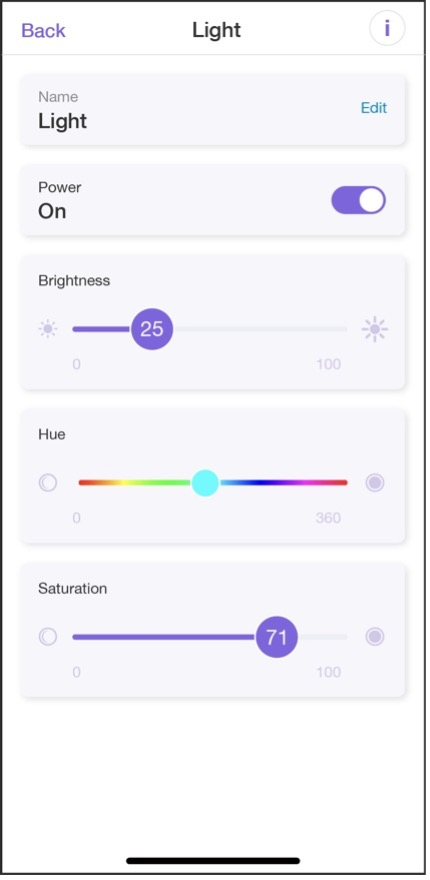
\includegraphics[width=0.33\textwidth]{D10Z/10-29}
    \caption{Bulb control interface}
\end{figure}

This section takes the control interface of light bulbs as an example, which contains the bulb's name, power on/off status, brightness, hue, and saturation. This information was obtained eariler when getting the list of bound devices in Section 10.6.2. The control interface for light bulbs is shown in Figure 10.29.

Given that one device might be controlled by different users, we should keep the device information in the smartphone app up to date by regularly refreshing and getting device status.

The API to get the status of a device is shown in Figure 10.30 and can be found at \url{https://swaggerapis.rainmaker.espressif.com/\#/Node\%20Parameter\%20Operations/getnodestate}.

\begin{figure}[ht]
    \centering
    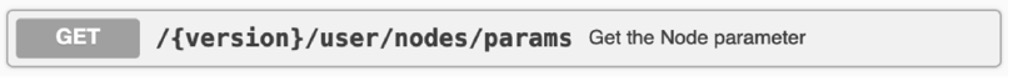
\includegraphics[width=0.8\textwidth]{D10Z/10-30}
    \caption{API to get device status}
\end{figure}

\begin{codebloc}
\begin{tabular}{d}
\verb|GET /v1/user/nodes/params?node_id=string|

\verb|Authorization: $accesstoken|
\end{tabular}
\end{codebloc}

In response to the “get status” request, the server returns:

\begin{codebloc}
\begin{tabular}{d}
\vspace{2pt}
\begin{verbatim}
{
        "Light": {
            "brightness": 0,
            "output": true
        },
        "Switch": {
            "output": true
        }
\end{verbatim}
\verb|}|
\end{tabular}
\end{codebloc}

Among the returned fields, \verb|Light| represents the brightness of the device, and \verb|bright-| \verb|ness| is the specific value; \verb|Switch| represents the on/off status of the device.

\textbf{Getting the device’s status in Android}

\note[Source code]{For the source code of getting device status in Android, please refer to \href{https://github.com/espressif/book-esp32c3-iot-projects/blob/main/phone_app/app_android/app/src/main/java/com/espressif/cloudapi/ApiManager.java}{\texttt{book-esp32c3-\newline iot-projects/phone\_app/app\_android/app/src/main/java/com/\newline espressif/cloudapi/ApiManager.java}}.}

\begin{codebloc}
\begin{tabular}{d}
\vspace{2pt}
\begin{verbatim}
1. public void getParamsValues(final String nodeId, final ApiResponseListener
2.  listener) {
3.      apiInterface.getParamValue(AppConstants.URL_USER_NODES_PARAMS,
4.            accessToken, nodeId).enqueue(new Callback<ResponseBody>() {
5.          @Override
6.          public void onResponse(Call<ResponseBody> call,
7.                                  Response<ResponseBody> response) {
8.              //Code Omitted
9.          }
10.         @Override
11.         public void onFailure(Call<ResponseBody> call, Throwable t) {
\end{verbatim}
\verb|12.             t.printStackTrace();|
\end{tabular}
\end{codebloc}

\begin{codebloc}
\begin{tabular}{d}
\vspace{2pt}
\begin{verbatim}
13.             listener.onNetworkFailure(new Exception(t));
14.         }
15.     });
\end{verbatim}
\verb|16. }|
\end{tabular}
\end{codebloc}

\vspace{6pt}
\textbf{Getting the device’s status in iOS}

\note[Source code]{For the source code of getting device status in iOS, please refer to \href{https://github.com/espressif/book-esp32c3-iot-projects/blob/cf25c67fbcedc44394fd7f90637b745d659f80ff/phone_app/app_ios/ESPRainMaker/ESPRainMaker/AWSCognito/ESPAPIManager.swift}{\texttt{book-esp32c3-iot-\newline projects/phone\_app/app\_ios/ESPRainMaker/ESPRainMaker/AWSCognito/\newline ESPAPIManager.swift}}.}

\begin{codebloc}
\begin{tabular}{d}
\vspace{2pt}
\begin{verbatim}
1.  func getDeviceParams(device: Device, completionHandler:
2.                      @escaping (ESPNetworkError?) -> Void) {
3.
4.      ESPExtendUserSessionWorker().checkUserSession(){accessToken, error in
5.          if let token = accessToken {
6.            let headers: HTTPHeaders = ["Content-Type": "application/json",
7.                                          "Authorization": token]
8.            let url = Constants.setParam + "?node_id=" +
9.                                          (device.node?.node_id ?? "")
10.           self.session.request(url, method: .get, parameters: nil,
11.                             encoding: JSONEncoding.default, headers:
12.                             headers).responseJSON { response in
13.                 //Code Omitted
14.           }
15.         } else {
16.           if self.validatedRefreshToken(error: error) {
17.                 completionHandler(.emptyToken)
18.           }
19.         }
20.     }
\end{verbatim}
\verb|21. }|
\end{tabular}
\end{codebloc}

\subsection{Changing Device Status}
The app allows users to change device name, power on/off status, brightness, hue, and saturation. This section will explain how to implement this function with the example of changing brightness and on/off status.

The API to change the status of a device is shown in Figure 10.31 and can be found at \href{https://swaggerapis.rainmaker.espressif.com/#/Node%20Parameter%20Operations/updatenodestate}{https://swaggerapis.rainmaker.espressif.com/\#/Node\%20Parameter\%20Operations/\newline updatenodestate}.

\begin{figure}[ht]
    \centering
    
\includegraphics[width=0.8\textwidth]{D10Z/10-31}
    \caption{API to change device status}
\end{figure}

\begin{codebloc}
\begin{tabular}{d}
\vspace{2pt}
\begin{verbatim}
1.  PUT /v1/user/nodes/params
2.  Authorization: $accesstoken
3.
4.  [
5.      {
6.          "node_id": "string",
7.          "payload": {
8.              "Light": {
9.                  "brightness": 100,
10.                 "output": true
11.             },
12.             "Switch": {
13.                 "output": true
14.             }
15.         }
16.     }
\end{verbatim}
\verb|17. ]|
\end{tabular}
\end{codebloc}

Among the returned fields, \verb|node_id| represents the device’s unique identifier; \verb|Light| represents the brightness of the device, and \verb|brightness| is the specific value; \verb|Switch| indicates the on/off status of the device.

\textbf{Changing device status in Android}

\note[Source code]{For the source code of changing device status in Android, please refer to \href{https://github.com/espressif/book-esp32c3-iot-projects/blob/main/phone_app/app_android/app/src/main/java/com/espressif/cloudapi/ApiManager.java}{\texttt{book-esp32c3-\newline iot-projects/phone\_app/app\_android/app/src/main/java/com/\newline espressif/cloudapi/ApiManager.java}}.}

\begin{codebloc}
\begin{tabular}{d}
\vspace{2pt}
\begin{verbatim}
1.  public void updateParamValue(final String nodeId,
2.                              JsonObject body, 
3.                              final ApiResponseListener listener) {
4.
5.      apiInterface.updateParamValue(AppConstants.URL_USER_NODES_PARAMS, 
6.                              accessToken, 
7.                              nodeId, 
8.                              body).enqueue(new Callback<ResponseBody>(){
9.          @Override
10.         public void onResponse(Call<ResponseBody> call,
11.                                 Response<ResponseBody> response) {
12.             //Code Omitted
\end{verbatim}
\verb|13.         }|
\end{tabular}
\end{codebloc}

\begin{codebloc}
\begin{tabular}{d}
\vspace{2pt}
\begin{verbatim}
14.
15.         @Override
16.         public void onFailure(Call<ResponseBody> call, Throwable t) {
17.             t.printStackTrace();
18.             listener.onNetworkFailure(new Exception(t));
19.         }
20.     });
\end{verbatim}
\verb|21. }|
\end{tabular}
\end{codebloc}

\vspace{6pt}
\textbf{Changing device status in iOS}

\note[Source code]{For the source code of changing device status in iOS, please refer to \href{https://github.com/espressif/book-esp32c3-iot-projects/blob/cf25c67fbcedc44394fd7f90637b745d659f80ff/phone_app/app_ios/ESPRainMaker/ESPRainMaker/AWSCognito/ESPAPIManager.swift}{\texttt{book-esp32c3-\newline iot-projects/phone\_app/app\_ios/ESPRainMaker/ESPRainMaker/\newline AWSCognito/ESPAPIManager.swift}}.}

\begin{codebloc}
\begin{tabular}{d}
\vspace{2pt}
\begin{verbatim}
1.  func setDeviceParam(nodeID: String?, parameter: [String: Any],
2.                      completionHandler: ((ESPCloudResponseStatus) ->
3.                      Void)? = nil) {
4.      NotificationCenter.default.post(Notification(name: Notification.Name
5.                                  (Constants.paramUpdateNotification)))
6.      if let nodeid = nodeID {
7.      ESPExtendUserSessionWorker().checkUserSession(){accessToken, error in
8.              if let token = accessToken {
9.                  let url = Constants.setParam + "?nodeid=" + nodeid
10.	                let headers: HTTPHeaders = ["Content-Type":
11.                                             "application/json", 
12.                                             "Authorization": token]
13.                 self.session.request(url, method: .put, 
14.                               parameters:
15.                               parameter, 
16.                               encoding: ESPCustomJsonEncoder.default,
17.                               headers: headers).responseJSON {response in
18.                     //Code Omitted
19.                 }
20.             } else {
21.                 let _ = self.validatedRefreshToken(error: error)
22.             }
23.         }
24.     }
\end{verbatim}
\verb|25. }|
\end{tabular}
\end{codebloc}

The code above allows users to change the status of a specific device. So far, we have implemented the functions of account registration, account login, device scanning, device connection, device provisioning, device binding, and remote control on RainMaker.

\section{Development of Scheduling and User Centre}
After implementing the core functional modules, it is also necessary to develop a scheduling module and a user centre module according to the functional requirements. Usually, these two modules are essential for a complete smartphone app. This section will describe the development of these two modules.

\subsection{Implementing Scheduling Function}
The scheduling interface is mainly used to show, create, and edit schedule events. The list page displays information such as name, time, date, and the recurring pattern of scheduled events. Each event has a toggle switch. The scheduling interface is shown in Figure 10.32.

\begin{figure}[ht]
    \centering
    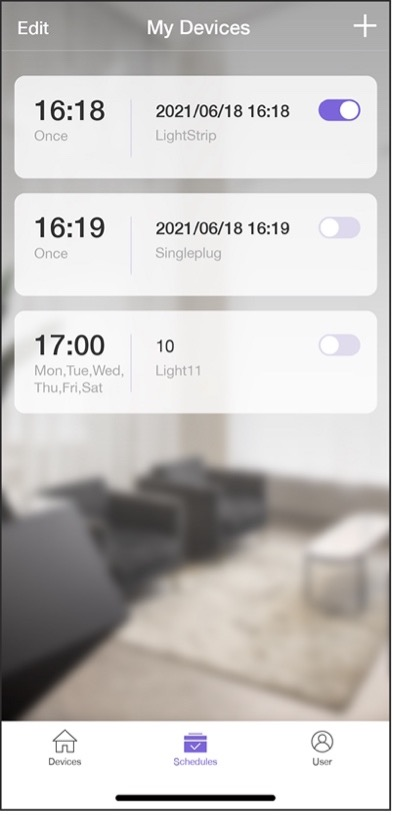
\includegraphics[width=0.3\textwidth]{D10Z/10-32}
    \caption{Scheduling interface}
\end{figure}

Data related to scheduling are stored in the local database of the smartphone app, and are added, deleted, modified, and queried there. See below for the code.

\textbf{Implementing scheduling in Android}

\note[Source code]{For the source code of implementing scheduling in Android, please refer to \href{https://github.com/espressif/book-esp32c3-iot-projects/blob/main/phone_app/app_android/app/src/main/java/com/espressif/ui/activities/AddScheduleActivity.java}{\texttt{book-\newline esp32c3-iot-projects/phone\_app/app\_android/app/src/main/java/com/\newline espressif/ui/activites/AddScheduleActivity.java}}.}

The code to save schedule data is as follows, where \verb|KEY_OPERATION decribes| the schedule event, \verb|KEY_ID| is the unique identifier, \verb|KEY_NAME| refers to the schedule’s name, \verb|KEY_DAYS| to the scheduled date, \verb|KEY_MINUTES| to the scheduled time, and \verb|KEY_TRIG|\newline \verb|GERS| to the recurring pattern (Monday to Friday).

\begin{codebloc}
\begin{tabular}{d}
\vspace{2pt}
\begin{verbatim}
1.  private void saveSchedule() {
2.      JsonObject scheduleJson = new JsonObject();
3.      scheduleJson.addProperty(AppConstants.KEY_OPERATION, "");
4.	
5.      //Schedule JSON
6.      scheduleJson.addProperty(AppConstants.KEY_ID, "");
7.      scheduleJson.addProperty(AppConstants.KEY_NAME, "");
8.
9.      JsonObject jsonTrigger = new JsonObject();
10.     jsonTrigger.addProperty(AppConstants.KEY_DAYS, "");
11.     jsonTrigger.addProperty(AppConstants.KEY_MINUTES, "");
12.	
13.     JsonArray triggerArr = new JsonArray();
14.     triggerArr.add(jsonTrigger);
15.     scheduleJson.add(AppConstants.KEY_TRIGGERS, triggerArr);
16.	
17.     prepareJson();
18.     //Code Omitted
\end{verbatim}
\verb|19. }|
\end{tabular}
\end{codebloc}

The code to update the schedule is as follows:

\begin{codebloc}
\begin{tabular}{d}
\vspace{2pt}
\begin{verbatim}
1.  @SuppressLint("CheckResult")
2.  Public void updateSchedules(final HashMap<String, JsonObject> map,
3.                              final ApiResponseListener listener) {
4.      //Code Omitted
\end{verbatim}
\verb|5.  }|
\end{tabular}
\end{codebloc}

\note[Source code]{For the source code of updating schedules in Android, please refer to \href{https://github.com/espressif/book-esp32c3-iot-projects/blob/main/phone_app/app_android/app/src/main/java/com/espressif/cloudapi/ApiManager.java}{\texttt{book-esp32c3-\newline iot-projects/phone\_app/app\_android/app/src/main/java/com/\newline espressif/cloudapi/ApiManager.java}}.}

%\vspace{6pt}
\textbf{Implementing scheduling in iOS}

\note[Source code]{For the source code of implementing scheduling in iOS, please refer to \href{https://github.com/espressif/book-esp32c3-iot-projects/blob/cf25c67fbcedc44394fd7f90637b745d659f80ff/phone_app/app_ios/ESPRainMaker/ESPRainMaker/Storage/ESPLocalStorageSchedules.swift}{\texttt{book-esp32c3-\newline iot-projects/phone\_app/app\_ios/ESPRainMaker/ESPRainMaker/Storage/\newline ESPLocalStorageSchedules.swift}}.}

The code to save schedule data is as follows, where \verb|KEY_OPERATION| decribes the schedule event, \verb|KEY_ID| is the unique identifier, \verb|KEY_NAME| refers to the schedule’s name, \verb|KEY_DAYS| to the scheduled date, \verb|KEY_MINUTES| to the scheduled time, and \verb|KEY_TRIGGERS| to the recurring pattern (Monday to Friday).

\begin{codebloc}
\begin{tabular}{d}
\vspace{2pt}
\begin{verbatim}
1.  func saveSchedules(schedules: [String: ESPSchedule]) {
2.      do {
3.          let encoded = try JSONEncoder().encode(schedules)
4.          saveDataInUserDefault(data: encoded, 
5.                              key: ESPLocalStorageKeys.scheduleDetails)
6.      } catch {
7.          print(error)
8.      }
\end{verbatim}
\verb|9.  }|
\end{tabular}
\end{codebloc}

The code to update the schedule is as follows:

\begin{codebloc}
\begin{tabular}{d}
\vspace{2pt}
\begin{verbatim}
1.  func fetchSchedules() -> [String: ESPSchedule] {
2.      var scheduleList: [String: ESPSchedule] = [: ]
3.      do {
4.          if let scheduleData = getDataFromSharedUserDefault(key:
5.                              ESPLocalStorageKeys.scheduleDetails) {
6.              scheduleList = try JSONDecoder().decode([String:
7.                              ESPSchedule].self, from: scheduleData)
8.          }
9.          return scheduleList
10.     } catch {
11.         print(error)
12.         return scheduleList
13.     }
\end{verbatim}
\verb|14. }|
\end{tabular}
\end{codebloc}

\subsection{Implementing User Centre}

The user centre module mainly includes functions like user profile, notification, change password, privacy policy, terms of use, documentation, voice services, and logout. The user centre interface is shown in Figure 10.33.

\begin{figure}[ht]
    \centering
    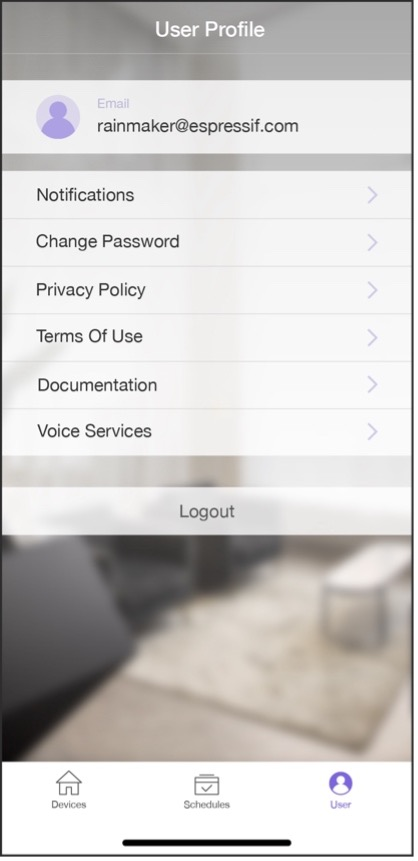
\includegraphics[width=0.3\textwidth]{D10Z/10-33}
    \caption{User centre interface}
\end{figure}

Among these functions, change password and logout need to be implemented by calling cloud APIs. In this section, we will take change password as an example of implementing user centre functions. The interface for changing password is shown in Figure 10.34.

\begin{figure}[ht]
    \centering
    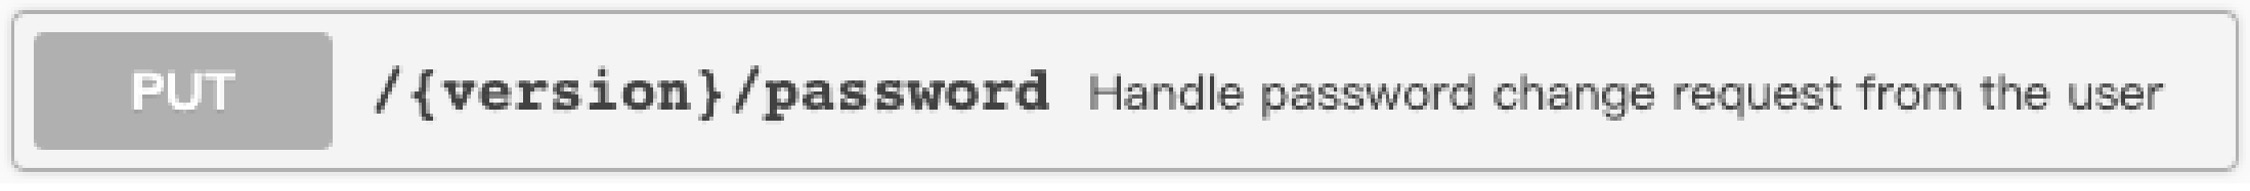
\includegraphics[width=0.8\textwidth]{D10Z/10-34}
    \caption{API for changing password}
\end{figure}

\begin{codebloc}
\begin{tabular}{d}
\vspace{2pt}
\begin{verbatim}
1.  PUT /v1/password
2.  Authorization: $accesstoken
3.  {
4.      "password": "password",
5.      "newpassword": "newpassowrd"
\end{verbatim}
\verb|6.  }|
\end{tabular}
\end{codebloc}

In the code above, \verb|password| refers to the old password, which aids the cloud in changing password; \verb|newpassword| refers to the new password. Once the password has been changed, the new password should come into use, and the old one becomes invalid.

In response to the request, the server returns:

\begin{codebloc}
\begin{tabular}{d}
\vspace{2pt}
\begin{verbatim}
1.  {
2.      "status": "success",
3.      "description": "Success description"
\end{verbatim}
\verb|4.  }|
\end{tabular}
\end{codebloc}

Among the returned fields, \verb|status| indicates the status of changing password; \verb|descrip|\newline \verb|tion| indicates the description of the change request.

\textbf{Changing password in Android}

\note[Source code]{For the source code of changing password in Android, please refer to \href{https://github.com/espressif/book-esp32c3-iot-projects/blob/main/phone_app/app_android/app/src/main/java/com/espressif/cloudapi/ApiManager.java}{\texttt{book-esp32c3-\newline iot-projects/phone\_app/app\_android/app/src/main/java/com/\newline espressif/cloudapi/ApiManager.java}}.}

\begin{codebloc}
\begin{tabular}{d}
\vspace{2pt}
\begin{verbatim}
1.  Public void changePassword(String oldPassword, String newPassword,
2.                              final ApiResponseListener listener) {
3.	
4.      JsonObject body = new JsonObject();
5.      body.addProperty(AppConstants.KEY_PASSWORD, oldPassword);
6.      body.addProperty(AppConstants.KEY_NEW_PASSWORD, newPassword);
7.	
8.      apiInterface.changePassword(AppConstants.URL_CHANGE_PASSWORD,
9.                              accessToken, 
10.                             body).enqueue(new Callback<ResponseBody>() {
11.	
12.         @Override
13.         public void onResponse(Call<ResponseBody> call,
14.                                 Response<ResponseBody> response) {
15.             //Code Omitted
16.         }
17.	
18.         @Override
19.         public void onFailure(Call<ResponseBody> call, Throwable t) {
20.             t.printStackTrace();
21.             listener.onNetworkFailure(new RuntimeException("Failed to
22.                                     change password"));
23.         }
24.     });
\end{verbatim}
\verb|25. }|
\end{tabular}
\end{codebloc}

\textbf{Changing password in iOS}

\note[Source code]{For the source code of changing password in iOS, please refer to \href{https://github.com/espressif/book-esp32c3-iot-projects/blob/cf25c67fbcedc44394fd7f90637b745d659f80ff/phone_app/app_ios/ESPRainMaker/ESPRainMaker/UserManagement/Interactors/ESPChangePasswordService.swift}{\texttt{book-esp32c3-iot-\newline projects/phone\_app/app\_ios/ESPRainMaker/ESPRainMaker/\newline UserManagement/Interactors/ESPChangePasswordService.swift}}.}

\begin{codebloc}
\begin{tabular}{d}
\vspace{2pt}
\begin{verbatim}
1.  func changePassword(oldPassword: String, newPassword: String) {
2.      sessionWorker.checkUserSession() { accessToken, sessionError in
3.        if let token = accessToken {
4.            self.apiWorker.callAPI(endPoint: .changePassword(url: self.url,
5.                                  old: oldPassword, new: newPassword,
6.                                  accessToken: token), encoding:
7.                                  JSONEncoding. default) { data, error in
8.                  self.apiParser.parseResponse(data, withError:
9.                                                  error) { umError in
10.                     self.presenter?.passwordChanged(withError: umError)
11.                 }
12.             }
\end{verbatim}
\verb|13.       } else {|
\end{tabular}
\end{codebloc}

\begin{codebloc}
\begin{tabular}{d}
\vspace{2pt}
\begin{verbatim}
14.        if !self.apiParser.isRefreshTokenValid(serverError:sessionError) {
15.                 if let error = sessionError {
16.                     self.noRefreshSignOutUser(error: error)
17.                 }
18.        } else {
19.                 self.presenter?.passwordChanged(withError: sessionError)
20.        }
21.       }
22.    }
\end{verbatim}
\verb|23. }|
\end{tabular}
\end{codebloc}

\subsection{More Cloud APIs}
In addition to the APIs detailed in the previous sections, RainMaker also provides some other APIs. Let’s have a quick look at them.

\textbf{Sharing devices with other users}

The API to share devices with other users is shown in Figure 10.35 and can be found at \href{https://swaggerapis.rainmaker.espressif.com/#/User%20Node%20Association/addUserNodeSharingRequests}{https://swaggerapis.rainmaker.espressif.com/\#/User\%20Node\%20Association/addUser\newline NodeSharingRequests}.

\begin{figure}[ht]
    \centering
    
\includegraphics[width=0.9\textwidth]{D10Z/10-35}
    \caption{API for sharing devices with other users}
\end{figure}

\textbf{Gettting the online/offline status of the device}

The API to get the online/offline status of the device is shown in Figure 10.36 and can be found at \href{https://swaggerapis.rainmaker.espressif.com/#/User%20Node%20Association/getNodeStatus}{https://swaggerapis.rainmaker.espressif.com/\#/User\%20Node\%20Association/\newline getNodeStatus}.

\begin{figure}[ht]
    \centering
    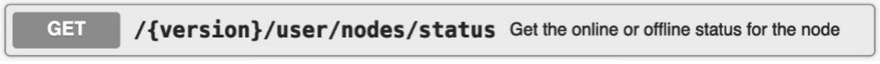
\includegraphics[width=0.9\textwidth]{D10Z/10-36}
    \caption{API for getting online/offline status of the device}
\end{figure}

\textbf{Creating device groups}

The API to create device groups is shown in Figure 10.37 and can be found at \url{https://swaggerapis.rainmaker.espressif.com/\#/Device\%20grouping/usercreatedevicegroup}.

\begin{figure}[ht]
    \centering
    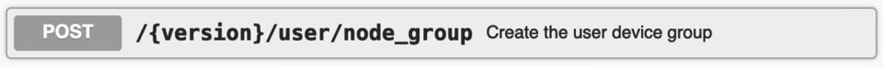
\includegraphics[width=0.9\textwidth]{D10Z/10-37}
    \caption{API for creating device groups}
\end{figure}

\textbf{Adding device to a group}

The API to add a device to a group is shown in Figure 10.38 and can be found at \url{https://swaggerapis.rainmaker.espressif.com/\#/Device\%20grouping/userupdatedevicegroup}.

\begin{figure}[ht]
    \centering
    
\includegraphics[width=0.9\textwidth]{D10Z/10-38}
    \caption{API for adding device to a group}
\end{figure}

\textbf{Deleting device groups}

The API to delete device groups is shown in Figure 10.39 and can be found at \url{https://swaggerapis.rainmaker.espressif.com/\#/Device\%20grouping/userdeletedevicegroup}.

\begin{figure}[ht]
    \centering
    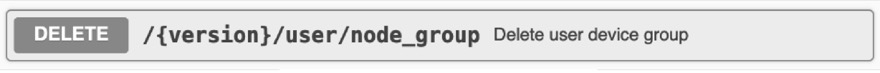
\includegraphics[width=0.9\textwidth]{D10Z/10-39}
    \caption{API for deleting device groups}
\end{figure}

Of course, RainMaker can do much more than what we have introduced. If interested, you may check the API documentation to discover more fun features!

\section{Summary}
This chapter has mainly presented how to develop a smartphone app. At the beginning, we introduced the development technologies for smartphone apps and the procedure to create a new smartphone app project, so as to give you a general picture of the entire development process. Then, we analysed the functional requirements for each module, namely user management, device provisioning, device control, and scheduling and user centre. At last, we detailed the development process of a smartphone app with source code, and showed how to implement device provisioning and control in the smartphone app.

\end{document}